\chapter{減偏極の解析}
本章では、積分効果、強度効果をレート方程式に取り込んだ上で図$\ref{HIMAC_data}$で表される偏極度推移に対してフィッティングを行い、
各緩和項の大きさを推定する。



\section{レート方程式}
飯沼・武田らは、Triplet-DNP による ${}^{1}\rm{H}$ スピン偏極率 $P$ の上昇の様子を、偏極生成
時定数 $T_D$ とレーザ照射時の偏極緩和時定数 $T_{1laser}$ を用いて、以下の式 \ref{eq:1} のような
レート方程式で表現できることを示した。
\begin{equation}
  \frac{dP(t)}{dt}=\frac{1}{T_D}(P_e-P(t))-\frac{1}{T_L}(P(t)-P_{th})
  \label{eq:1}
\end{equation}
ここで、$P_e$ は電子スピンの偏極率、$Pt_h$ は ${}^1\rm{H}$ スピンの熱平衡状態の偏極率である。ま
た、$T_{1laser}$ は ${}^1\rm{H}$ スピンのスピン-格子緩和時間 $T_1$ と、${}^1\rm{H}$ スピンとの偏極交換に使われ
なかった残留偏極電子による緩和 $T_e$ を用いて以下の式\ref{eq:2}ように表せる。

\begin{equation}
  \frac{1}{T_{1laser}}=\frac{1}{T_1}+\frac{1}{T_e}
  \label{eq:2}
\end{equation}

本実験条件では Pth は非常に小さいため、Pth を無視して式$\ref{eq:1}$を解くと以下の解を得る。

\begin{equation}
  P(t)=\frac{P_e}{1+\frac{T_D}{T_{1laser}}}\left[1-\rm{exp} \left(-\left(\frac{1}{T_D}+\frac{1}{T_{1laser}}\textit{t}\right)\right)\right]
  \label{eq:3}
\end{equation}

放射損の効果として以下の強度効果と積分効果を仮定した。\\
・強度効果:ビーム照射下の標的温度が上昇し、スピン格子緩和時間が減少する\\

・積分効果:ビーム照射によってC-H結合が外れて不対電子が現れ、偏極緩和要因となる\\

\begin{figure}[h]
  \centering
  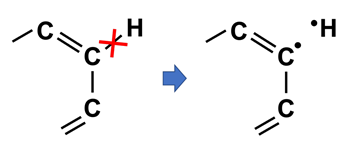
\includegraphics[width= 7cm]{./chap3/fig/CCbond.png}
  \caption{ビーム照射時のC-H結合切断による不対電子の発生}
  \label{fig:CCbond}
\end{figure}

強度効果をビーム強度に比例する項、積分効果をビーム強度、照射時間に比例する項として式\ref{eq:4}のように取り入れた。
また、ビームのon/off切り替えや強度変更の際、温度が平衡に達するのに有限の時間を要することを考慮し、強度効果には補正を行った。
この微分方程式は解析解を持たないため、数値計算を用いる。

\begin{equation}
  \frac{dP}{dt}=\frac{1}{T_D}(P_e-P(t))-\left(\frac{1}{T_L}+\alpha I t_{beam}+\beta\left[1-\exp\left(-\frac{t_{switch}}{\gamma}\right)\right]\right)P(t)
  \label{eq:4}
\end{equation}
ここで、$\alpha$は積分効果の寄与の大きさを表す係数、$\beta$は強度効果の寄与の大きさを表す係数、$\gamma$は温度が平衡に達するまでの時間スケールを表す係数である。
また、$t_{beam}$はビームの照射時間、$t_{switch}$はビーム照射のon/off切り替えや強度変更時刻からの経過時間を表す。
上式は解析的に解くことができないため、数値計算を用いてHIMAC実験で得られた偏極度推移の
データに対してフィッティングを行うことで、積分効果と強度効果の相対評価を行う。

\section{解析手法}
パラメータ探索には以下の3つの手法を検討し、最も精度よくフィットできたPSO法を採用した。
\begin{enumerate}
  \item Grid Search
  \item Levenberg-Marquardt(LM)法
  \item 粒子群最適化(PSO)法(Particle Swarm Optimize)
\end{enumerate}


\section{解析結果}
\begin{figure}[h]
  \centering
  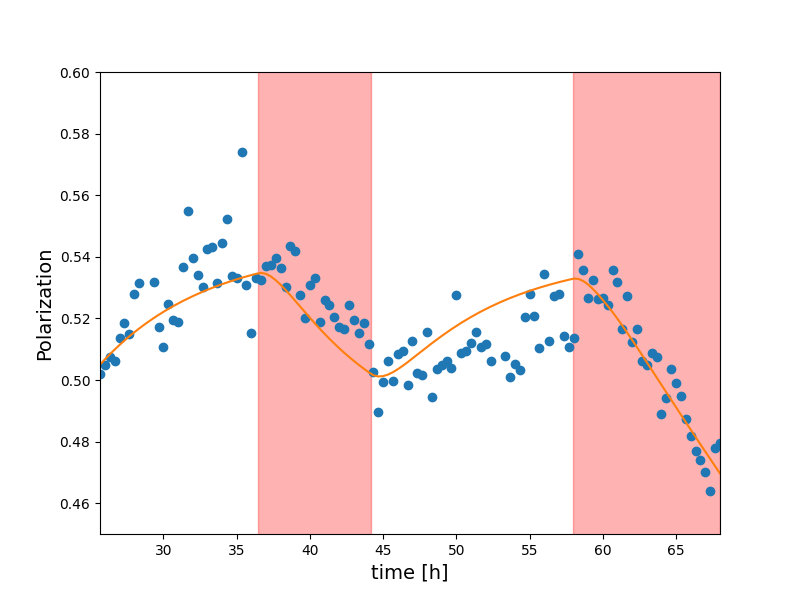
\includegraphics[width= 13cm]{./chap3/fig/fit.png}
  \caption{実験データ(点)と最適パラメータを用いた時のフィット結果(実線)}
  \label{fit}
\end{figure}
PSO法によるフィッティングの結果、図$\ref{fit}$のような曲線が得られた。計算条件を表にまとめた。計算回数及び粒子数は表の値より大きくした場合でもχ2に有意な変化(PSOの性質上、初期パラメータのとり方によるわずかなχのずれが存在する)が確認できなかったため、計算時間を考慮し、この値とした。
\begin{table}[]
  \begin{tabular}{|l|l|}
  \hline
  パラメータ数   & 6   \\ \hline
  粒子数      & 100 \\ \hline
  繰り返し回数   & 30  \\ \hline
  ローカル項重み  & 0.5 \\ \hline
  グローバル項重み & 0.9 \\ \hline
  慣性項重み    & 0.1 \\ \hline
  \caption{計算条件}
  \end{tabular}
  \end{table}

\begin{table}[]
  \begin{tabular}{|l|l|l|}
  \hline
               & min   & max   \\ \hline
  $\rm{T_D}$ {[}h{]} & 12    & 12.5  \\ \hline
  $\rm{T_L}$ {[}h{]} & 18    & 20.5  \\ \hline
  $\rm{P_0}$         & 0.49  & 0.505 \\ \hline
  $\rm{\alpha}$        & $1e^{-16}$ & $1e^{-14}$ \\ \hline
  $\rm{\beta}$         & $1e^{-4}$  & $1e^{-3}$  \\ \hline
  $\rm{\gamma}$        & 70    & 80    \\ \hline
  \caption{パラメータ探索範囲}
  \end{tabular}
  \end{table}

\section{各パラメータの数値}
\begin{table}[h]
  \begin{tabular}{|l|l|}
  \hline
  $\rm{T_D}$    & 12.288            \\ \hline
  $\rm{T_L}$    & 18.609            \\ \hline
  $\rm{P_0}$    & 0.505             \\ \hline
  $\alpha$ & 3.788e-15         \\ \hline
  $\beta$  & 2.548e-04         \\ \hline
  $\gamma$ & 76.36218400202554 \\ \hline
  \caption{フィッティング結果}
  \end{tabular}
  \end{table}

誤差の取り扱いまでは行えていないため、表には誤差なしで表記している。



% \chapter{偏極${}^3$He標的装置}
% 本章では、陽子--$^3$He弾性散乱実験による$^3$He偏極分解能測定のために我々のグループが開発した偏極$^3$He標的装置について述べる。偏極$^3$He標的装置は主に以下の項目に分けられる。
% %
% \begin{itemize}
%  \item $^3$Heガスを封入する標的セル
%  \item 標的セルの製作装置
%  \item 偏極生成装置
%  \item $^3$He偏極度測定装置
% \end{itemize}
% %
% 図\ref{pol-sys}に我々のグループが開発した偏極$^3$He標的の概略図を示す。標的部は$^3$HeガスとN$_2$ガスおよびRbが封入された標的セルと、Rb蒸気を発生させるためにセルを加熱する標的オーブンから構成される。また偏極生成装置は静磁場を発生させるメインコイル、光ポンピングに使用される半導体レーザー、円偏光レーザーを生成するための光学系から構成される。$^3$He偏極度測定装置は、AFP-NMR装置および本研究で開発したRb-ESR測定装置の二つに分けられる。AFP-NMR装置は高周波磁場を発生させるドライブコイル、メインコイルに電流を流し、かつ電流値を掃引できるコイル用電源、NMR信号を読み出すためのピックアップコイルおよび測定系から構成される。Rb-ESR測定装置は$D_2$線の蛍光を検出するためのフォトダイオード、ESRを起こすための振動磁場を加えるESRコイルおよび測定系から構成される。以下では、これらの装置について詳細に述べる。

% \begin{figure}[tbp]
%  \centering
%  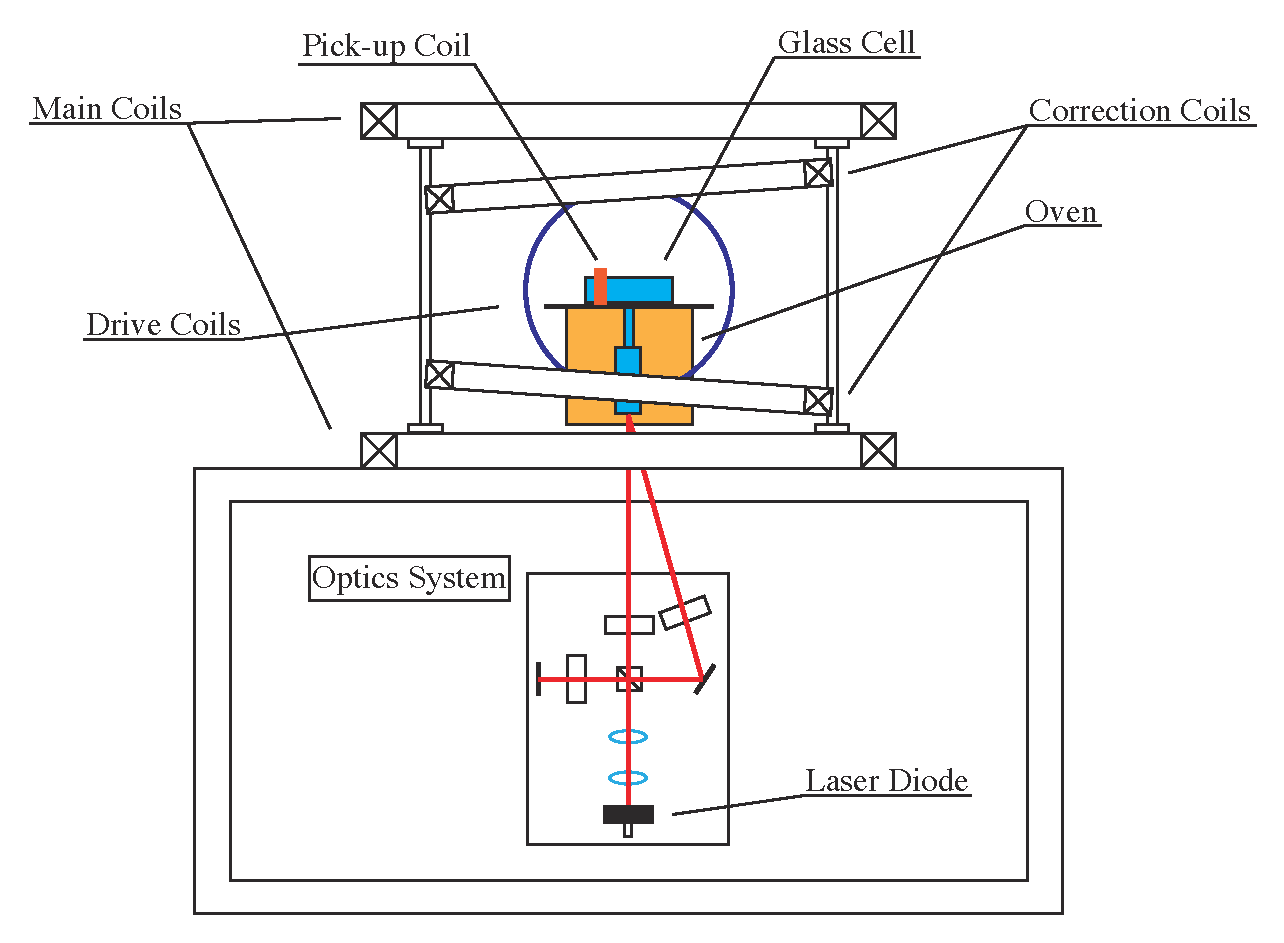
\includegraphics[clip,width=11cm]{./chap3/fig/pol-sys_sche.pdf}\\
%  \caption{偏極$^3$He標的の概略図}
%  \label{pol-sys}
% \end{figure}

% %%%% 3.1 %%%%
%  \section{${}^3$He標的セル}
%  \label{sec:tar_cell}
% 我々は、陽子--$^3$He弾性散乱実験に用いる標的として、$^3$Heガスをガラスセルに封入した標的セルを製作した。ガラスセルの素材としてはGeneral Electric社のアルミノ珪酸ガラスであるGE180を用いた。GE180は、ガラス中に含まれる磁性不純物の量が少ないため、不純物との相互作用による$^3$Heの核スピンの偏極緩和率が小さいことが知られている\cite{Jia13}。またCorning社のpyrexガラス等に比べ、$^3$Heガスの透過率が低く、長期間高密度の状態を維持することが可能である。\\
%  我々のグループが製作した標的セルの典型的な形状を図\ref{kuki}に示す。標的セルは、散乱実験でビームを照射する標的部とRb蒸気を発生させるためにオーブンに入れるポンピング部から成るダブルセル構造である。$^3$He原子核は、ポンピング部でRbとのスピン交換によって偏極し、その後拡散することで標的部へと移動する。この時Rb蒸気も標的部に移動しないように、標的部およびポンピング部を繋ぐ管は$\phi10~{\rm mm}$の外径かつ$65~{\rm mm}$の長さにしてある。また$3$気圧の高密度の$^3$Heガスを想定し、ガラスセルの厚さは約$1~{\rm mm}$とした。標的部のビーム入射面および出射面は、入射ビームのエネルギー損失を出来るだけ小さくするために約$0.5~{\rm mm}$の厚さとし、また強度を高めるために半球形に凹ませている。

% \begin{figure}[tbp]
%  \centering
%  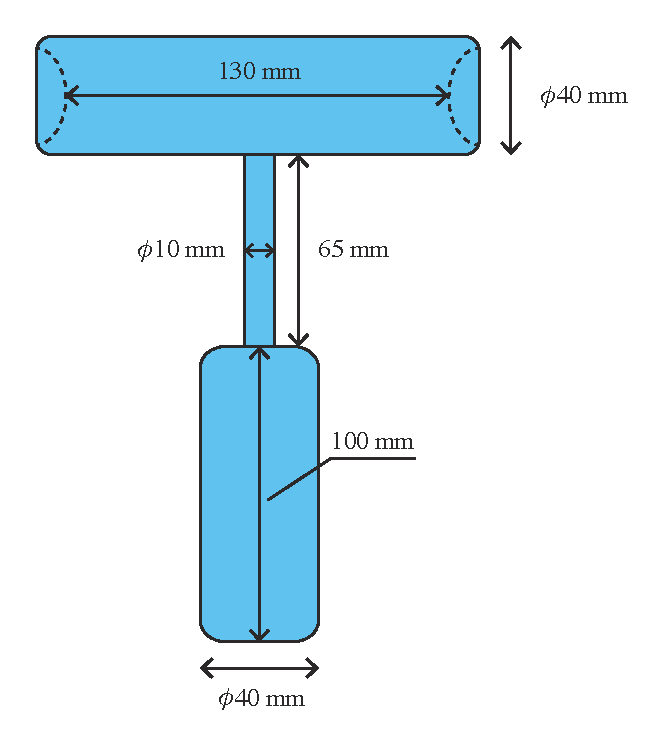
\includegraphics[clip,width=6cm]{./chap3/fig/kuki_sche.pdf}\\
%  \caption{製作したセルの典型的な形状}
%  \label{kuki}
% \end{figure}

% 以下の節では、この標的セルの製作装置および製作方法について述べる。

% %% 3.1.1 %%
%   \subsection{標的セルの製作装置}
% SEOP法によって$^3$He原子核を偏極させるためには、$^3$Heガスの他にRbおよびN$_2$ガスをガラスセルに封入する必要がある。また2.3.2節でも述べたように、$^3$He原子核の偏極度を高めるためには$^3$He原子核の偏極緩和率を小さくすることが重要である。従って、ガラスセルの洗浄や真空引き、ベーキング等によってセル内部の不純物を取り除くことが必要である。\\
%  標的セルの製作装置の模式図を図\ref{vac-sys}に示す。セル製作装置は、ガラスセルが繋がれているセルブランチ、真空引きを行うためのロータリーポンプおよびターボ分子ポンプ(TMP)、真空度を測定するためのバラトロンゲージやクリスタルゲージおよびペニングゲージ、そして$^3$HeガスやN$_2$ガスを純化して導入するためのゲッターから構成される。

% \begin{figure}[tbp]
%  \centering
%  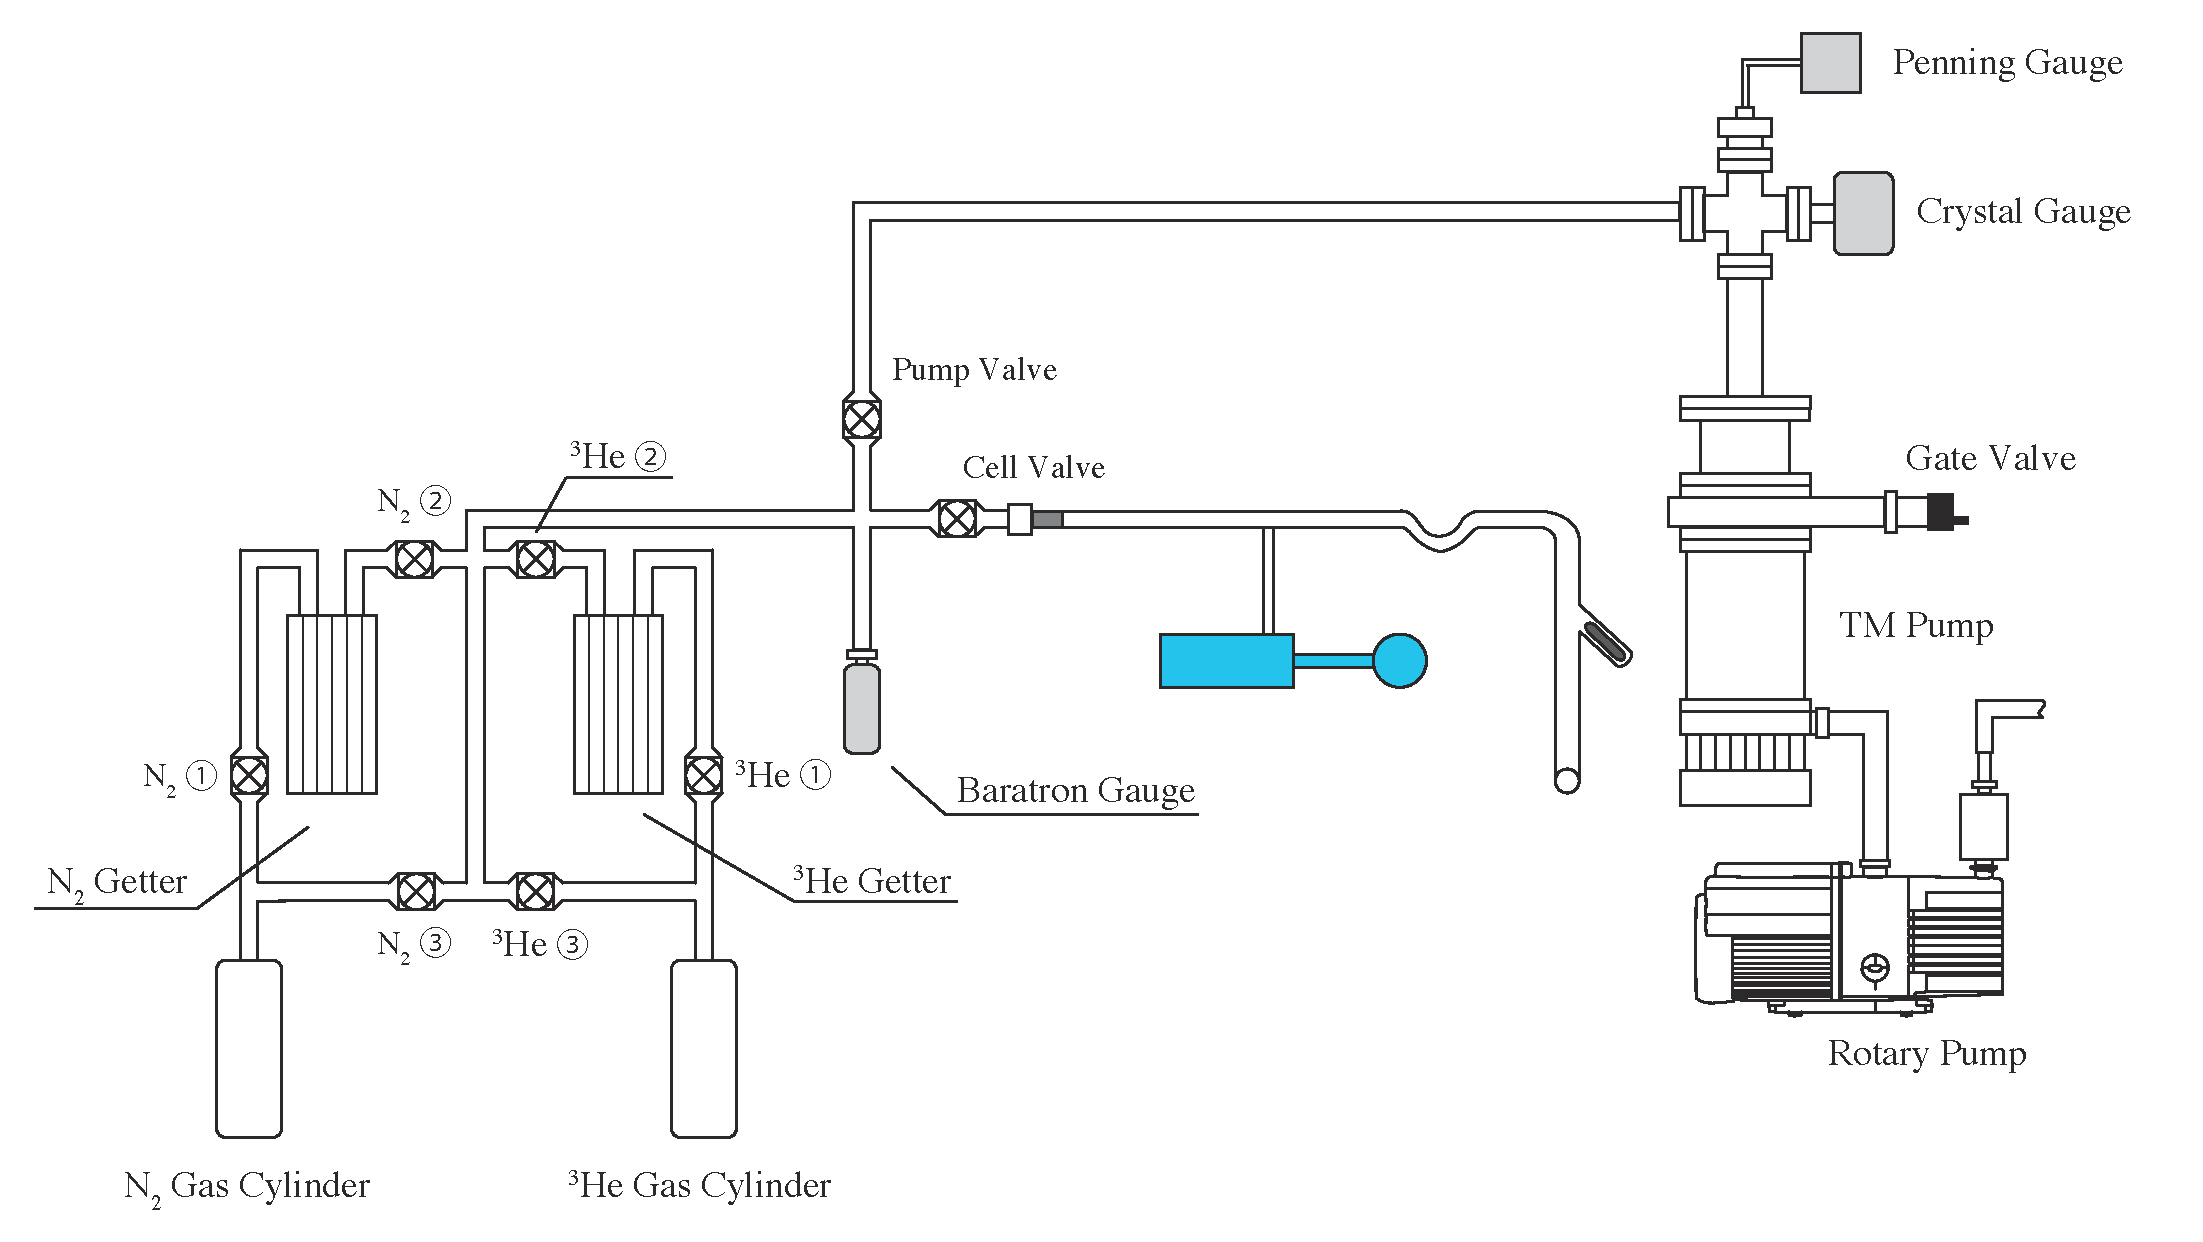
\includegraphics[clip, width=1.0\linewidth]{./chap3/fig/vacuum-sys.pdf}\\
%  \caption{標的セル製作装置の模式図}
%  \label{vac-sys}
% \end{figure}

% \begin{figure}[tbp]
%  \centering
%  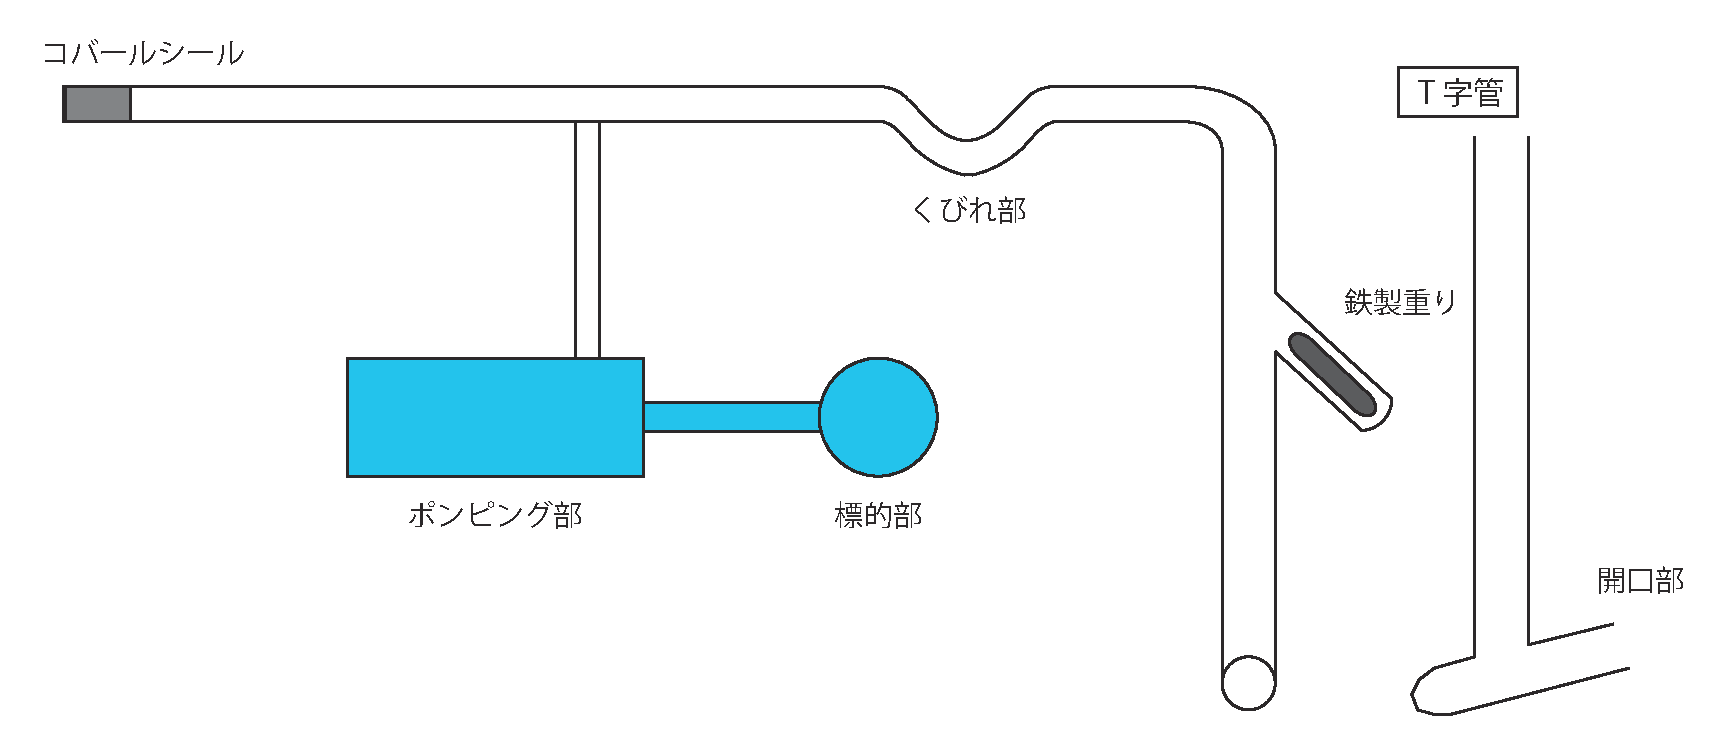
\includegraphics[clip, width=1.0\linewidth]{./chap3/fig/cell-branch.pdf}\\
%  \caption{セルブランチの概略図。水色の領域は標的セルの部分。}
%  \label{cell-bra}
% \end{figure}

% セルブランチの概略図を図\ref{cell-bra}に示す。標的セルは初めセルブランチに繋がれており、端にコバールシールを溶接して真空排気系と接続している。標的セルの素材であるGE180はバーナー等による加工が難しいため、標的セル以外の部分は比較的加工が容易であるpyrexガラスを使用した。標的セルとセルブランチとは$\phi8~{\rm mm}$のガラス管で接続されており、このガラス管を通して真空引きや洗浄液の流入による標的セル内の洗浄を行う。またセルブランチの“T字管”部分には、純度$99.9%$のRb $1~{\rm g}$が入ったアンプル(93-3736, STREM社)を導入するための開口部がある。開口部からRbアンプルを入れてバーナーで封じ切った後、鉄芯を磁石で持ち上げて落とすことでアンプルを割る。鉄芯は、セル内の高真空度を保つためにpyrexガラスで包まれている。\\
%  セルブランチの真空引きは、ロータリーポンプ(RV-12, EDWARDS社)およびターボ分子ポンプ(TMP280, 島津製作所)によって行う。これらの真空排気系による典型的な到達真空度は$4.5 \times 10^{-5}~{\rm Pa}$である。\\
%  真空度はクリスタルゲージ(M-320XG, キャノンアネルバ社)およびペニングゲージ(TPG300, BALZERS社)によって測定した。クリスタルゲージは水晶振動子の共振インピーダンスが圧力に応じて変化する性質を利用した真空計で、$10^5〜10^{-2}~{\rm Pa}$の範囲の圧力を測定できる。またペニングゲージは真空中に残留する気体を電離させ、それによって生成されるイオンや電子を電極で捕集することで流れる電流から圧力を測定する真空計である。クリスタルゲージよりも高い真空度を測定でき、およそ$10^{-9}~{\rm Pa}$の低圧力まで測定が可能である。\\
%  $^3$HeガスおよびN$_2$ガスを標的するに封入する時の圧力は、バラトロンゲージ(750B, mks社)によって測定した。バラトロンゲージは差圧によって薄い金属膜を変形させ、それに応じて変化する静電容量の値から圧力を測定する真空計であり、大気圧のおよそ$10^{-2}$倍から$10^2$倍までの範囲の圧力を測定できる。またバラトロンゲージは、圧力に対応した電圧値を出力するので、圧力の較正を行う必要がある。図\ref{bara_calib_fig}に、バラトロンゲージの較正結果を示す。横軸はアネロイド気圧計(7610-20, 佐藤計量器製作所)で測定した圧力、縦軸はバラトロンゲージの出力電圧値を示している。一次関数でフィッティングした結果、圧力$Prs$に対するバラトロンゲージの出力電圧値$V_{\rm bara}$の関係は
% %
% \begin{equation}
%  V_{\rm bara}~[{\rm V}] = (1.513 \pm 0.003) \times 10^{-3} Prs~[{\rm hPa}] - (0.5 \pm 1.0) \times 10^{-3}
%  \label{bara_calib}
% \end{equation}
% %
% となった。

% \begin{figure}[tbp]
%  \centering
%  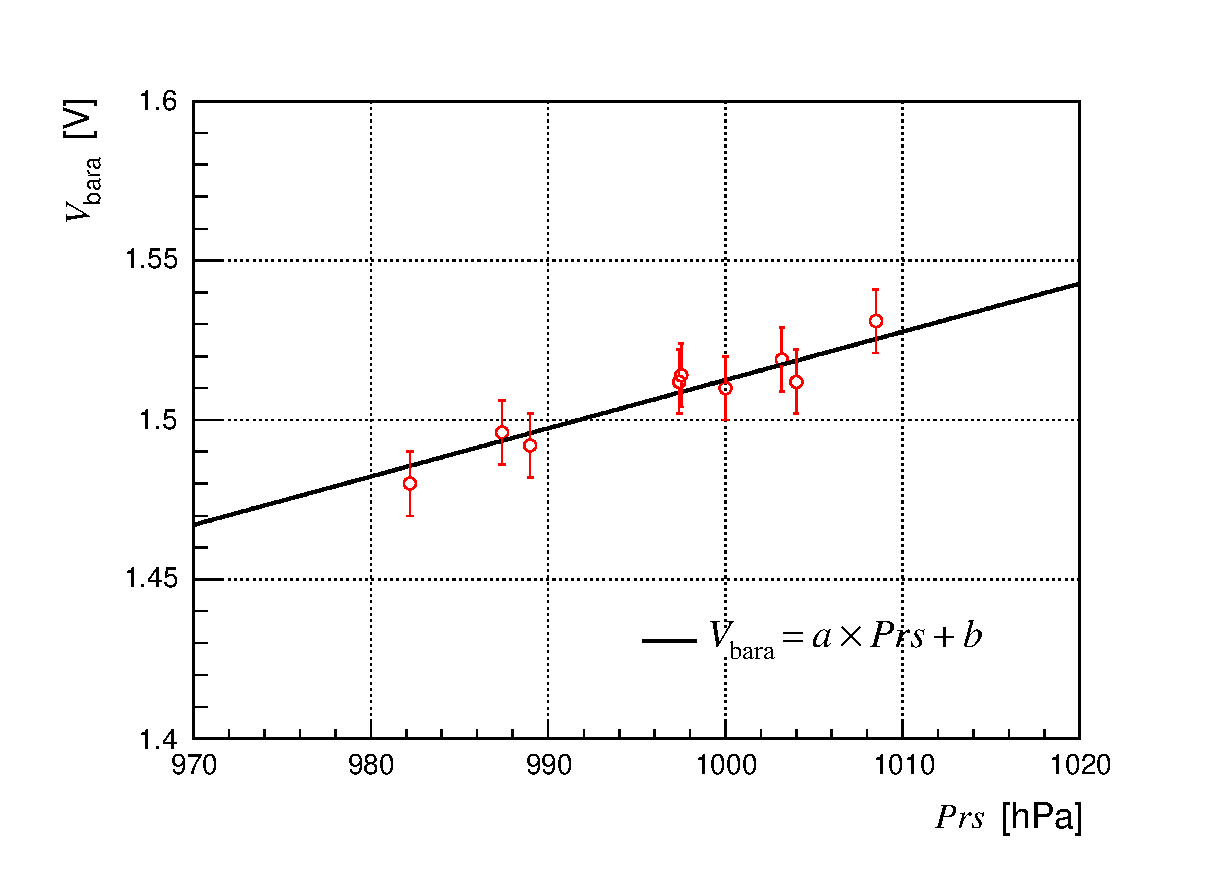
\includegraphics[clip, width=10cm]{./chap3/fig/Bara_calib.eps}\\
%  \caption{バラトロンゲージの較正結果}
%  \label{bara_calib_fig}
% \end{figure}

% 標的セルに$^3$HeガスおよびN$_2$ガスを封入する際は、ゲッターを通して不純物を除去し、純化させる。ゲッターはsaes gettes社のGC50(He用:PS2-GC50-R-1, N$_2$用:PS2-GC50-N-1)を用いた。これによって、$^3$Heガスは$99.999%$、N$_2$ガスは$99.999999%$までの純度にすることが可能である。

% %%%%%%%

% %% 3.1.2 %%
%   \subsection{標的セルの製作方法}
% 上記のセル製作装置を用いて、標的セルの製作を行った。セル製作の手順を以下に示す。
% %
% \begin{itemize}
%  \item ガラスセルの洗浄
%  \item Rbアンプル導入
%  \item ベーキングおよびRbアンプル割り
%  \item Rbの移送
%  \item $^3$HeガスおよびN$_2$ガス封入
% \end{itemize}
% %
% 以下では、これらの項目それぞれについて述べる。
% %
% \begin{description}
%  \item[ガラスセルの洗浄]  
%  %
%  \begin{enumerate}
%   \item セル内の金属化合物や油脂等を取り除くために、$10%$程度に希釈した中性洗剤を用いて洗浄する。 希釈した洗剤溶液を$50℃$程度まで温め、セルブランチを約6時間浸す。この時、1時間毎にセルブランチ内の洗剤溶液の入れ替えを行う。
%   \item 純水で5回以上すすぎ、洗剤溶液を洗い流す。
%   \item アセトンで3回以上すすぎを行う。
%   \item エタノールで3回以上すすぎを行う。
%  \end{enumerate}
%  %
% \end{description}
% %
% \begin{description}
%  \item[Rbアンプル導入]  
%  %
%  \begin{enumerate}
%   \item セルブランチの洗浄後、真空排気系に接続する。この時、ガスラインにN$_2$ガスを充填させておく。これによって、接続時に不純物が真空排気系に流入するのを防ぐ。
%   \item N$_2$ボンベを開け、セルブランチのT字管の開口部からN$_2$ガスが流れ出るようにする。
%   \item ヒートガンでT字管を加熱し、エタノールを蒸発させる。
%   \item Rbアンプルを開口部から投入し、N$_2$ボンベを閉じて開口部をバーナーで封じ切る。
%   \item セルバルブおよびポンプバルブを開け、真空引きを開始する。
%   \item 再びヒートガンで加熱して、セルブランチ内のエタノールを蒸発させ取り除く。
%   \item 10時間程度真空引きを行う。
%  \end{enumerate}
%  %
% \end{description}
% %
% \begin{description}
%  \item[ベーキングおよびRbアンプル割り]  
%  %
%  \begin{enumerate}
%   \item Rbアンプル以外の部分にリボンヒーターを巻き、約$235℃$まで加熱しベーキングを行う。
%   \item 3日間程度ベーキングを行う。
%   \item ベーキングを停止し、ポンプバルブを閉じる。
%   \item セルブランチに$1$気圧程度N$_2$ガスを充填する。
%   \item 磁石で鉄芯を持ち上げ落とし、Rbアンプルを割る。
%   \item アンプル内の不活性ガスを取り除くために、ポンプバルブを開けて再びベーキングおよび真空引きを行う。
%   \item 真空度が$\sim 10^{-5}~{\rm Pa}$程度になるまでベーキングおよび真空引きを続ける。
%  \end{enumerate}
%  %
% \end{description}
% %
% \begin{description}
%  \item[Rbの移送]  
%  %
%  \begin{enumerate}
%   \item ベーキングを停止し、セルブランチが常温程度まで冷えるのを待つ。
%   \item くびれ部を送風で冷やしながら、T字管にリボンヒーターを巻いて加熱し、Rbをくびれ部に移送する。
%   \item くびれ部に十分な量のRbが溜まったら、ポンプバルブを閉じる。
%   \item セルブランチ内に$1$気圧程度N$_2$ガスを充填し、T字管をバーナーで切り落とす。
%   \item ポンプバルブを開け、くびれ部以外の部分にリボンヒーターを巻き、ベーキングおよび真空引きを行う。
%   \item 真空度が$\sim 10^{-5}~{\rm Pa}$程度になるまでベーキングおよび真空引きを続ける。
%   \item ヒートガンで加熱し、標的セル内にRbを移送する。
%   \item 10時間程度真空引きを行う。
%  \end{enumerate}
%  %
% \end{description}
% %
%  \begin{description}
%  \item[$^3$HeガスおよびN$_2$ガス封入]  
%  %
%  \begin{enumerate}
%   \item ポンプバルブを閉じ、真空引きを停止する。
%   \item 標的セルを液体窒素に浸し、標的セル内部の温度を窒素の沸点($=-195.8℃$)まで冷却する。
%   \item N$_2$ボンベを開け、セルブランチ内にガスを送る。この時、GC50を通過させてガスを純化する。
%   \item バラトロンゲージの圧力を読みながら、常温でN$_2$ガスの圧力が約$100~{\rm Torr}$となるように調整する。
%   \item セルバルブを閉じ、ポンプバルブを開けて真空排気系の真空引きを行う。
%   \item ポンプバルブを閉じ、$^3$Heボンベを開けてセルブランチ内にガスを導入する。この時、N$_2$ガス同様GC50を通過させてガスを純化する。
%   \item バラトロンゲージの圧力を読みながら、$^3$Heガス圧力が$1$気圧程度になるよう調整する。これによって、常温で$^3$Heガス圧力が約$3$気圧となる。
%   \item バーナーで標的セルとセルブランチを繋いでいるガラス管を封じ切る。
%  \end{enumerate}
%  %
% \end{description}
% %
% 以上の過程により、陽子--$^3$He弾性散乱実験で使用する標的セル“Kuki”を製作した。
 
% %%%%%%%
% %%%%%%%%%%

% %%%% 3.2 %%%%
%  \section{偏極生成装置}
% $^3$He原子核の偏極生成装置は、静磁場を発生させるためのメインコイルおよび補正コイル、Rb蒸気を発生させるためにガラスセルを加熱する標的オーブン、Rbの光ポンピングのための半導体レーザーおよび光学系から構成される。本節では、これらの装置それぞれについて述べる。

% %% 3.2.1 %%
%   \subsection{静磁場発生用コイル}
% スピンの量子化軸を決めるための静磁場は、メインコイルおよび補正コイルの二組のコイルによって発生させている。メインコイルは、標的セル周辺の領域での静磁場の均一度を高めるために、ヘルムホルツ型のコイルを採用している。補正コイルは図\ref{pol-sys}のようにヘルムホルツコイルを上下に少し傾けたものであり、メインコイルによって作られる静磁場の均一度を調整するために用いられる。メインコイルおよび補正コイルの仕様を表\ref{coils}に示す。メインコイルは、数 Aの電流で$1〜3~{\rm mT}$の静磁場を発生させることができる。この時発生させる静磁場の向きは鉛直下向きである。また発生させる静磁場の均一度は、ヘルムホルツコイルの中心から標的セルの長さである$15~{\rm cm}$の領域において$10^{-3}~{\rm cm^{-1}}$程度である。
% %
%  \begin{table}[htbp]
%   \caption{メインコイルおよび補正コイルの仕様}
%   \centering
%   \begin{tabular}{|c||c|c|} \hline
% & メインコイル & 補正コイル \\ \hline
% 直径 & $100~{\rm cm}$ & $75~{\rm cm}$ \\
% 導線の太さ & $\phi 1.7~{\rm mm}$ & $\phi 1.7~{\rm mm}$ \\
% 巻き数 & 300 回 & 100 回 \\ \hline
%   \end{tabular}
%   \label{coils}
%  \end{table}\\
% %
%  メインコイルに流れる電流$I_{\rm main}$と中心部におけるメインコイルが作る静磁場の$z$成分$B_z$の関係を図\ref{main-coil}に示す。図\ref{main-coil}のグラフは、最小二乗法によって一次関数でフィッティングした結果を示している。フィッティングの結果、$I_{\rm main}$と$B_z$の関係式は
% %
% \begin{equation}
%  B_z~[{\rm mT}] = (0.498 \pm 0.016) \times I_{\rm main}~[{\rm A}] - (0.091 \pm 0.062)
%  \label{Bz-Imain}
% \end{equation}
% %
% となった。およそ$6~{\rm A}$の電流を流すことによって、$3~{\rm mT}$程度の静磁場を発生させることができる。メインコイルおよび補正コイルの電源は工藤電機製の直流電源(作番 030058)を用いた。この直流電源はTTL規格のトリガー信号を入力することで、設定された二つの電流値の間を掃引させることができる。

% \begin{figure}[tbp]
%  \centering
%  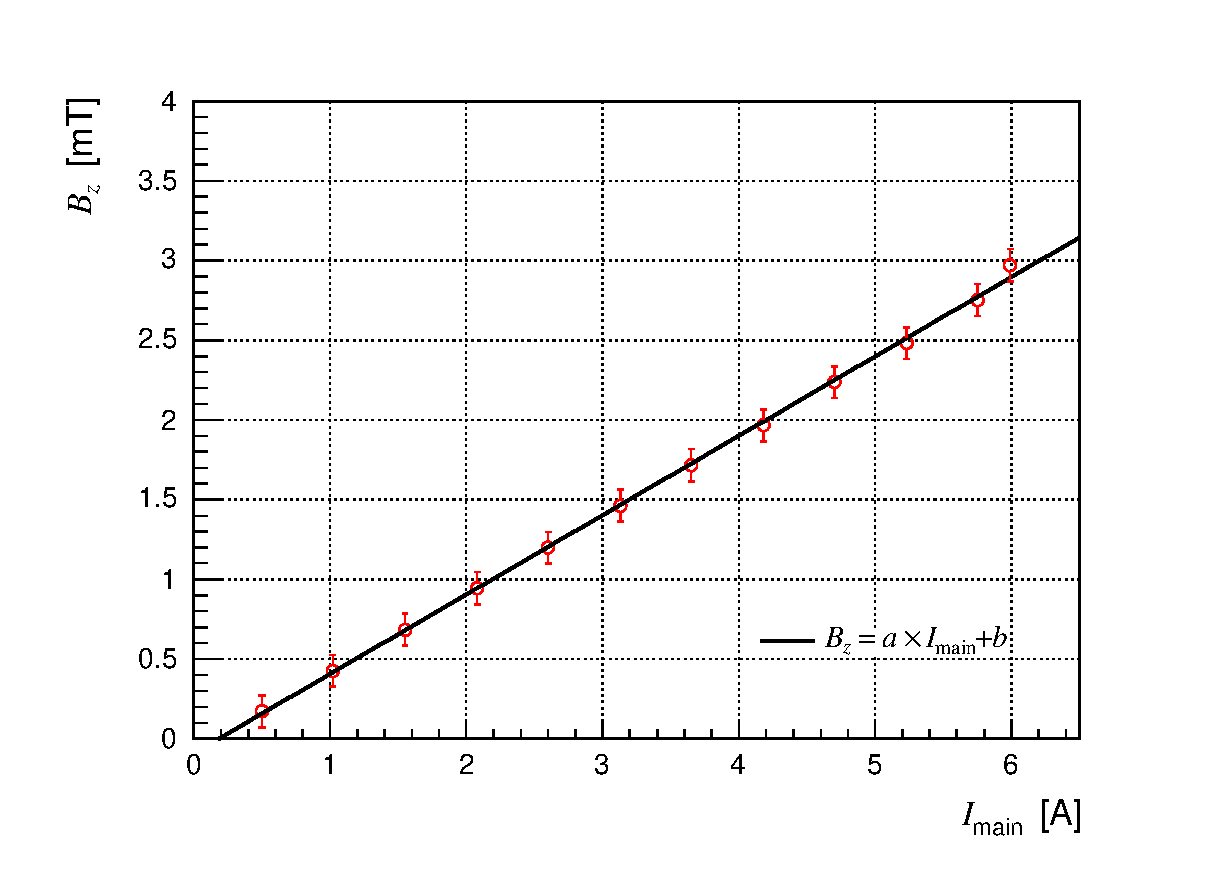
\includegraphics[clip, width=10cm]{./chap3/fig/Main_Coil.eps}\\
%  \caption{メインコイルの励磁曲線}
%  \label{main-coil}
% \end{figure}

% %%%%%%%

% %% 3.2.2 %%
%   \subsection{標的オーブン}
% 標的セル内のポンピング部に光ポンピングするにあたって十分な量のRb蒸気を発生させるためには、ポンピング部を$200$℃程度の高温にまで加熱する必要がある。そこで、標的セルのポンピング部のみを標的オーブン内に入れ、熱風によって加熱させる方法を取った。標的オーブンの材質は、非磁性かつ高い耐熱性を持つポリエーテルエーテルケトン(PEEK)を採用した。標的オーブンの模式図を図\ref{oven}に示す。オーブンのビーム軸方向の側面および底面はガラス窓が取り付けられており、下方向からガラス窓を通してレーザーを照射する。オーブン内は、ポンピング部の側面にアルミ製のダクトを通して熱風機(Hot-Wind System, LEISTER社)から熱風を送ることで高温に保つ。また熱風機の出す熱風の温度および風量は外部信号入力による制御が可能であり、ファンクションジェネレーター(FG120, YOKOGAWA社)からの出力を外部入力信号として用いた。ファンクションジェネレーターはLinuxコンピューターによるGPIB制御で動作させており、これによって標的オーブン内の温度を一定に保つようにした。標的オーブン内の温度は白金測温抵抗体(Pt100)を用いて測定した。

% \begin{figure}[tbp]
%  \centering
%  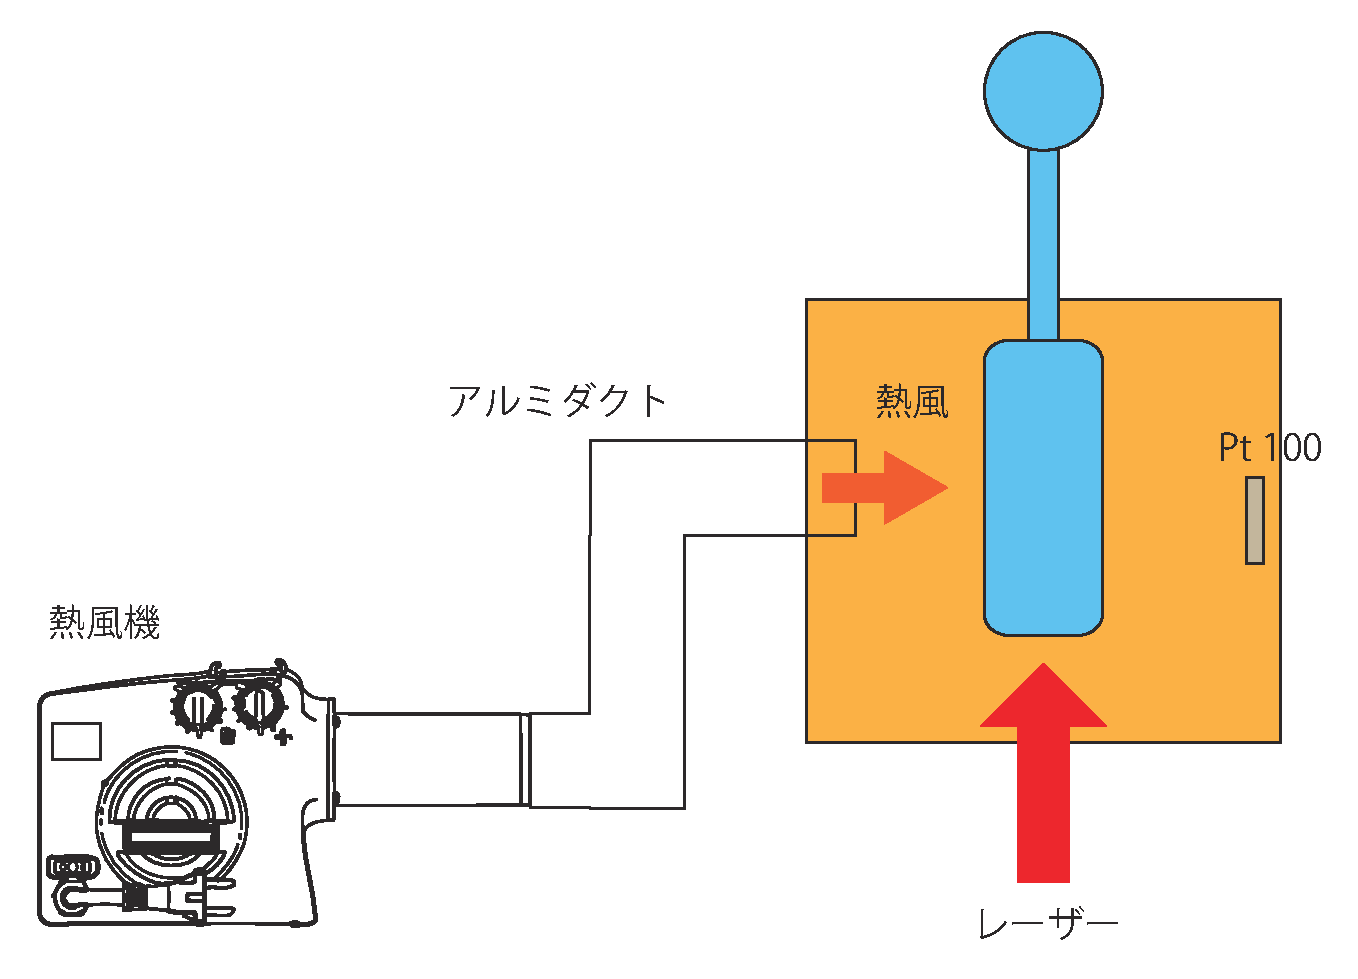
\includegraphics[clip, width=8cm]{./chap3/fig/oven_sche.pdf}\\
%  \caption{標的オーブンの模式図}
%  \label{oven}
% \end{figure}

% %%%%%%%

% %% 3.2.3 %%
%   \subsection{半導体レーザー}
% 光ポンピングによってRb原子を偏極させるためのレーザーとして、ファイバー結合型高出力半導体レーザー(FAP-79-30C-800-B, COHERENT社)を用いた。半導体レーザー本体は二つのレーザーアレイパッケージで構成されており、それぞれのレーザーアレイには光ファイバーが結合されている。またこれらの二つのファイバーはひとつにまとめられ、単一のファイバー端子として使用することができる。本研究で使用した半導体レーザーの仕様を表\ref{LD}に示す。半導体レーザーの電源はLumina Power社のLDD-250-4-6を用い、二つのレーザーアレイに対し直列に繋いだ。
% %
%  \begin{table}[htbp]
%   \caption{半導体レーザーの仕様}
%   \centering
%   \begin{tabular}{|c|c|} \hline
% 中心波長 & $795~{\rm nm}$ \\
% FWHM & ${< 4~\rm nm}$ \\
% 最大出力& $30~{\rm W}$ \\
% ファイバーコア径 & $800~{\rm \mu m}$ \\
% 開口数 & $< 0.16$ \\ \hline
%   \end{tabular}
%   \label{LD}
%  \end{table}\\
% %
%  本研究で使用した半導体レーザーの励起曲線を図\ref{laser-pow}に示す。図\ref{laser-pow}において、横軸はレーザー電源の出力電流、縦軸はパワーメーター(PM150-50, Molectron社)で測定したレーザー出力である。レーザーは電源の供給電流$8~{\rm A}$程度から発振し始め、その後は供給電流に対して線形に出力が増加していく。供給電流に対するレーザー出力の比はおよそ$1.14~{\rm W/A}$である。

% \begin{figure}[tbp]
%  \centering
%  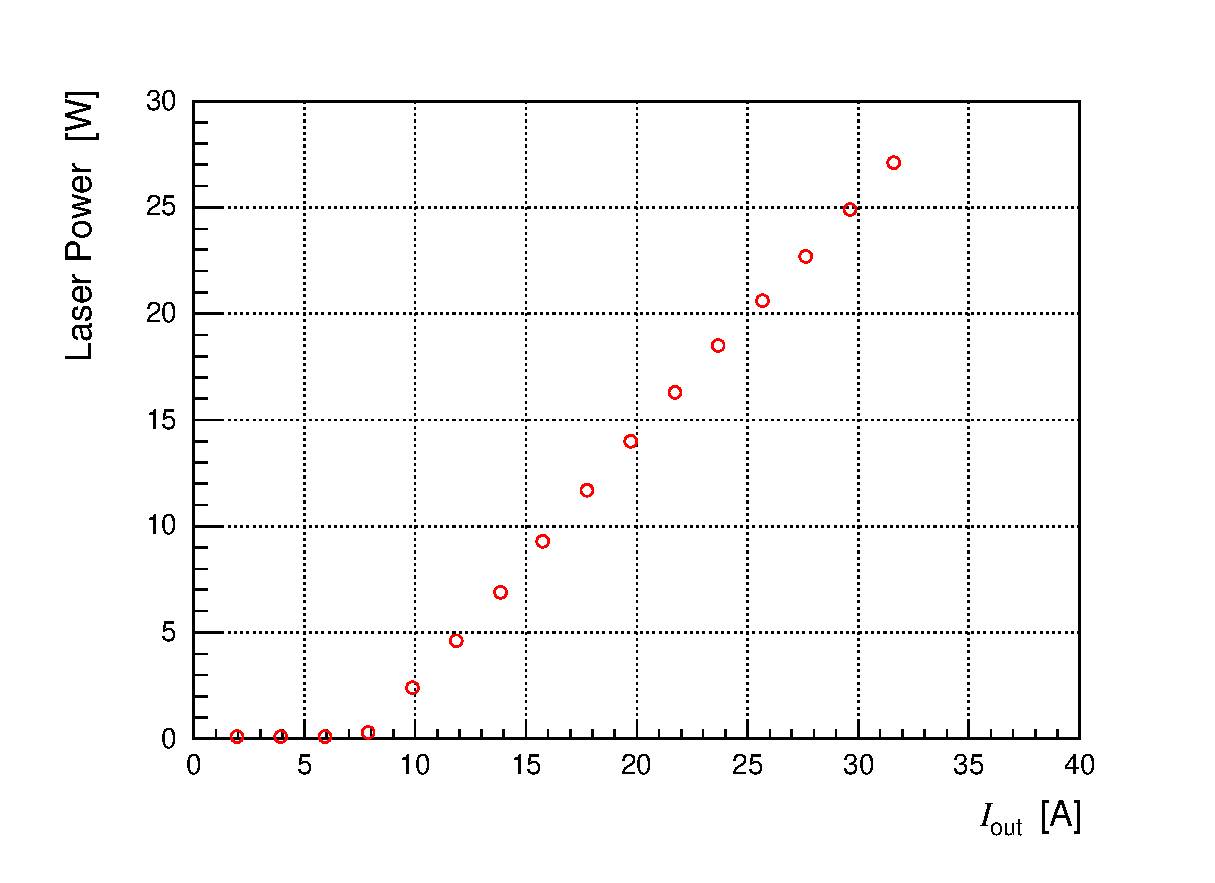
\includegraphics[clip, width=10cm]{./chap3/fig/Laser_Pow-Iout.eps}\\
%  \caption{半導体レーザーの励起曲線}
%  \label{laser-pow}
% \end{figure}

% 半導体のバンドギャップおよび光共振器として用いる半導体結晶の劈開面の距離は温度に依存する。よって、レーザー素子の温度を調整することで発振するレーザー波長を変化させることができる。そこでレーザー本体の温度を制御するために、レーザー本体を排気扇付きの空冷箱に固定し、銅板を介してPeltier素子を取り付けた。Peltier素子は、二種類の金属の接合部に電流を流すと、一方の金属からもう一方の金属へと熱が伝導していくPeltier効果を利用した半導体素子で、流す電流値を調整することでレーザー本体の温度を調整できる。レーザー本体の温度は、温度センサー(LM335)をレーザー本体に取り付け測定した。またPeltier素子に電流を流す直流電源(E3642A, Agilent社)をGPIB制御で動作させることにより、レーザー本体の温度を調整および安定させた。\\
%  レーザーの中心波長が$795~{\rm nm}$になるレーザー温度を確認するために、定期的にレーザー波長の温度依存性測定を行った。典型的なレーザー温度に対するレーザー波長の測定結果を図\ref{laser_wl}に示す。レーザーの波長はADVANTEST社のデジタル光波長計(TQ8325)を用いて測定した。測定結果から、レーザー温度を$31$℃にすることで波長が$795~{\rm nm}$となることが分かる。

% \begin{figure}[tbp]
%  \centering
%  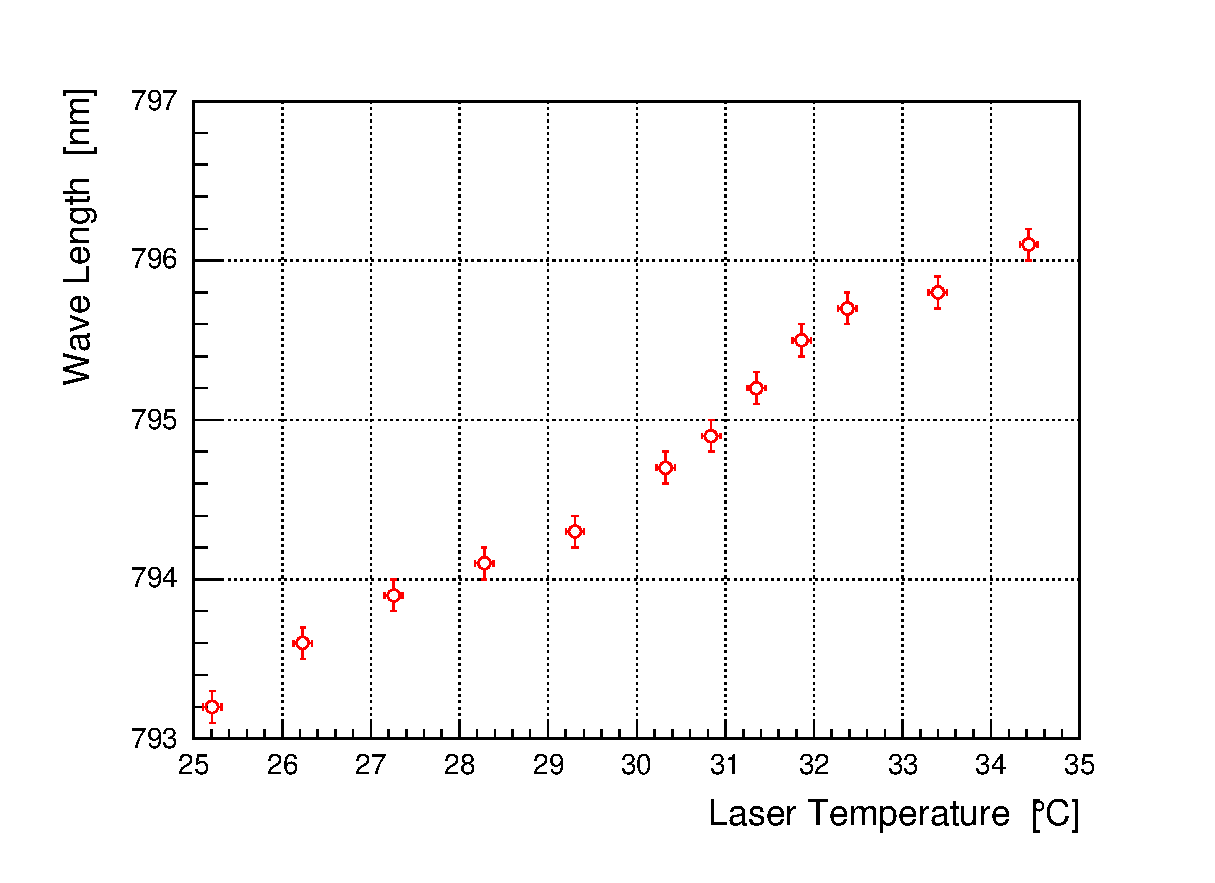
\includegraphics[clip, width=10cm]{./chap3/fig/Laser_wl.eps}\\
%  \caption{半導体レーザーの波長の温度依存性}
%  \label{laser_wl}
% \end{figure}

% %%%%%%%

% %% 3.2.4 %%
%  \subsection{光学系}
% 光ポンピングによってRb原子を偏極させるためには、円偏光レーザーを照射する必要がある。しかし、光ファイバーからのレーザー光は偏光を保存せず、非偏光状態である。そこで、偏光ビームスプリッター(PBS)や1/4波長板($\lambda/4$板)を用いて円偏光を生成するための光学系を組んだ。本研究で用いた光学系の模式図を図\ref{laser-sys}に示す。PBSは二つの直角プリズムにより構成される光学素子で、接合面にコーティングされた誘電体多層膜により入射した光をその偏光方向によって反射もしくは透過させる。そのため、図\ref{laser-sys}においてレーザーファイバーから照射された光は、PBSによって透過光であるP偏光(偏光方向が紙面に対して平行)の光と、反射光であるS偏光(偏光方向が紙面に対して垂直)の光に分けられる。透過光および反射光は1/4波長板を透過して標的セルへと照射される。1/4波長板は異方性媒質の結晶によって構成される光学素子で、直交する進相軸および遅相軸を透過した直線偏光の間で$\pi/2$の位相差を生じさせる。よって、直線偏光を両軸に対して入射角度が$45^\circ$となるように入射させれば円偏光を生成することができる。

% \begin{figure}[tbp]
%  \centering
%  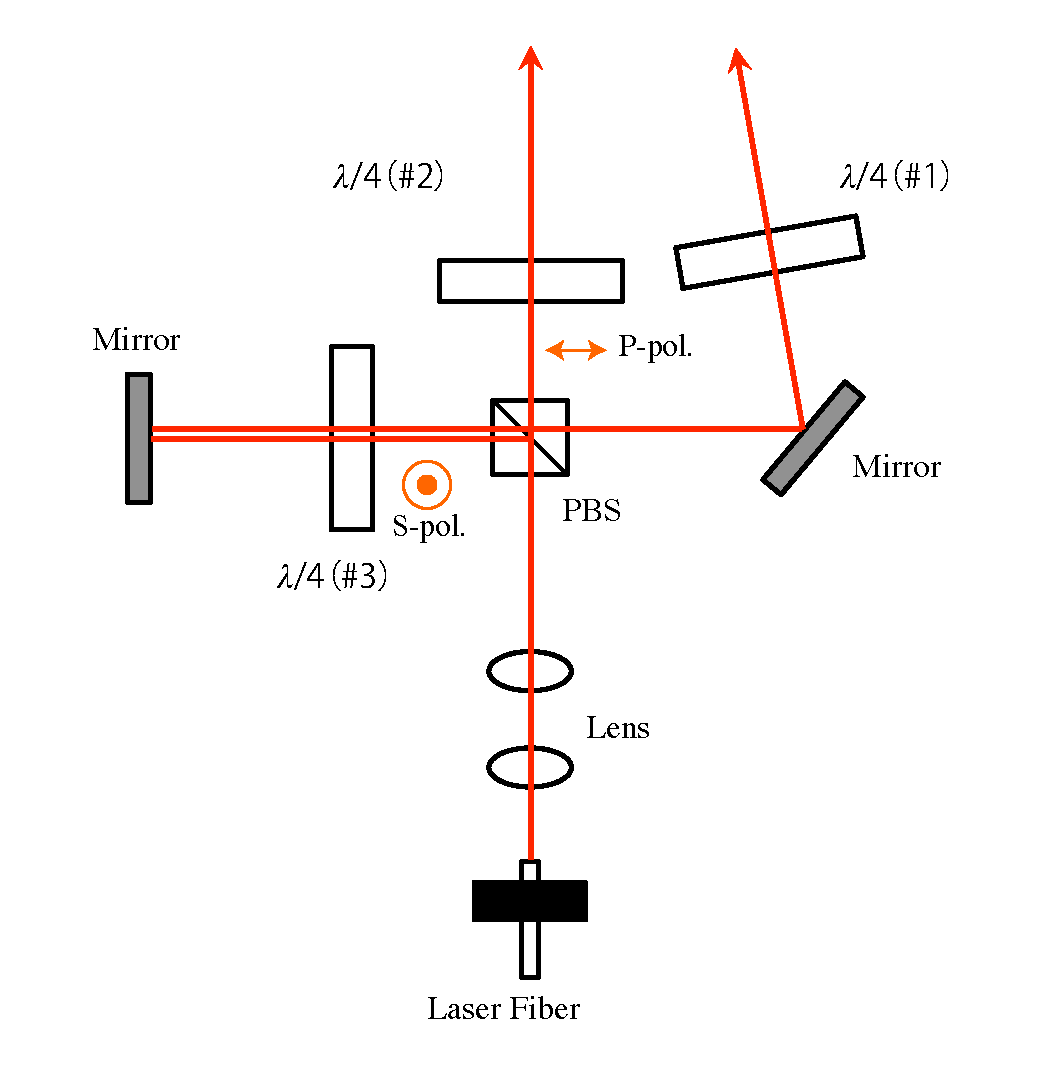
\includegraphics[clip, width=8cm]{./chap3/fig/laser-sys.pdf}\\
%  \caption{円偏光を生成するための光学系の模式図}
%  \label{laser-sys}
% \end{figure}

% PBSによって分離された直線偏光を1/4波長板を透過させて円偏光を生成する際、1/4波長板の角度の最適化が重要である。角度の調整は、図\ref{laser-sys}において1/4波長板の直後にPBSを置き、PBSを透過したレーザーの出力をパワーメーターで測定することで行う。PBSは前述のようにP偏光のみを透過させるため、1/4波長板通過前のレーザーがP偏光である場合は直線偏光となっている時に出力が最大、それに対して円偏光となっている時に出力が最小となる。また1/4波長板通過前のレーザーがS偏光である場合は直線偏光となっている時に出力が最小、円偏光となっている時に出力が最大となる。すなわち、1/4波長板の光軸周りの角度$\theta$に対応し、PBS透過後のレーザー出力は$1/2(1 \pm \cos^2 \theta)$に比例することになる。ここで、$+$はP偏光、$-$はS偏光を表す。\\
%  図\ref{laser-sys}において、\#2および\#3の1/4波長板通過後のレーザーに対して、PBS透過後のレーザー出力の測定結果を図\ref{lam4_2_3}に示す。この測定から、\#2および\#3の1/4波長板の角度を$49^\circ$および$139^\circ$にすることで円偏光が生成されることを確認した。また\#3の1/4波長板の角度を$139^\circ$に設定し、\#1の1/4波長板について同様の測定を行った。測定結果を図\ref{lam4_1}に示す。\#1の1/4波長板に関しても、同様に$49^\circ$および$139^\circ$にすることで円偏光の生成を確認した。よって、\#1、\#2および\#3の1/4波長板の角度は全て$49^\circ$または$139^\circ$に設定し、円偏光のレーザーによる光ポンピングを行う。

% \begin{figure}[tbp]
%  \centering
%  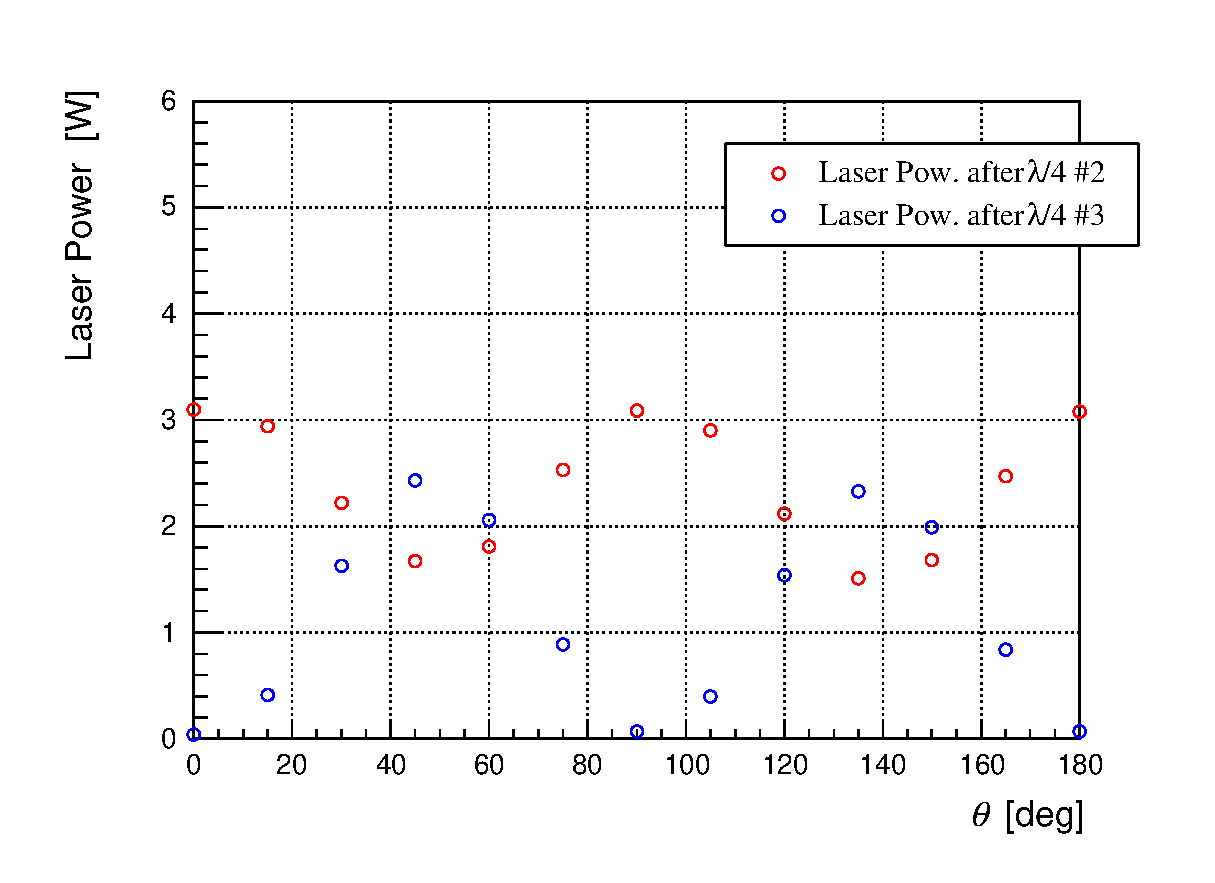
\includegraphics[clip, width=10cm]{./chap3/fig/lam4_2_3_Pow.eps}\\
%  \caption{1/4波長板の光軸周りの角度$\theta$に対するPBS透過光強度(\#2および\#3)}
%  \label{lam4_2_3}
% \end{figure}

% \begin{figure}[tbp]
%  \centering
%  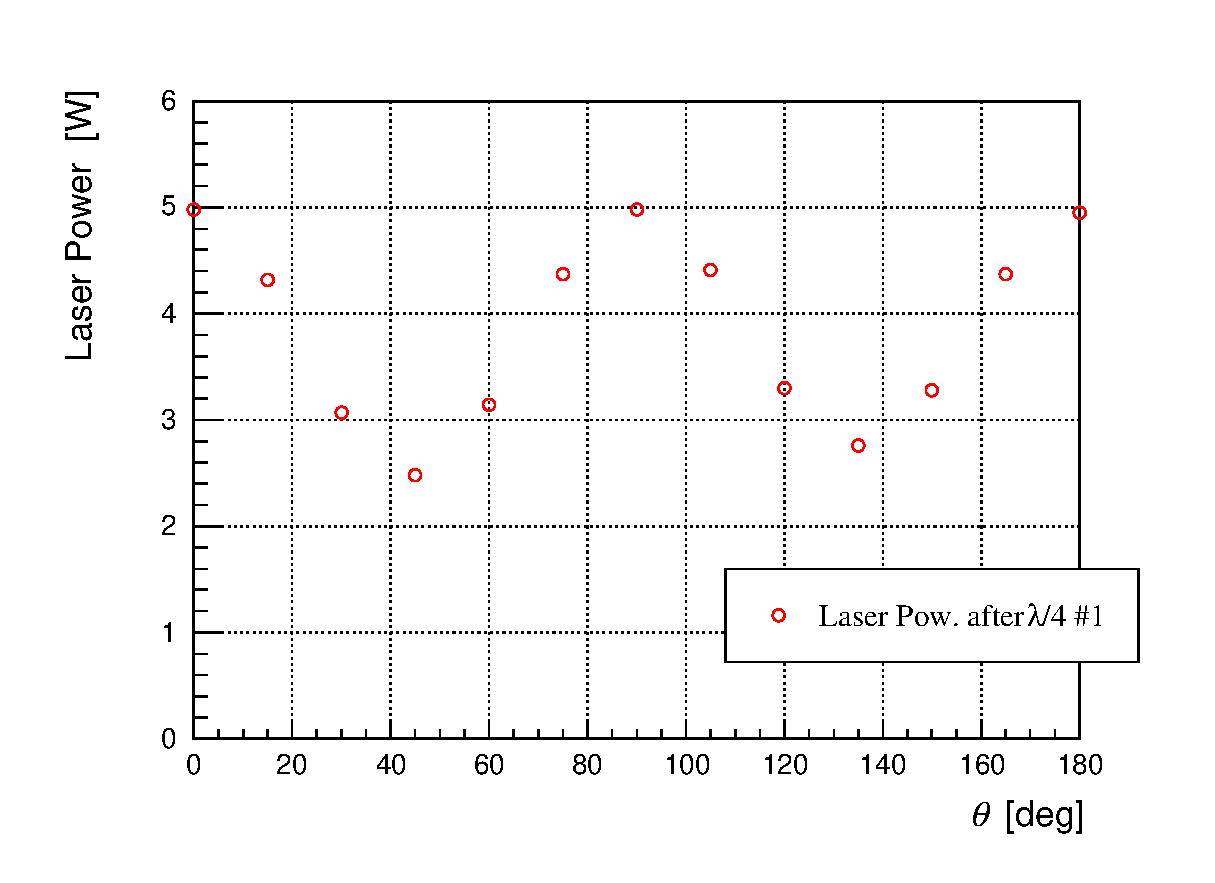
\includegraphics[clip, width=10cm]{./chap3/fig/lam4_1_Pow.eps}\\
%  \caption{1/4波長板の光軸周りの角度$\theta$に対するPBS透過光強度(\#1)}
%  \label{lam4_1}
% \end{figure}

% %%%%%%%
% \newpage
% %%%% 3.3 %%%%
%  \section{${}^3$He偏極度測定装置}
% SEOP法によって偏極した$^3$He原子核の偏極度測定法として、散乱実験中も測定を行えるAFP-NMR法を採用し、また$^3$He偏極度の絶対値較正のためにRbのESR周波数シフト測定システムを開発した。本節では、これらの$^3$He偏極度測定を行うための測定装置について述べる。

% %% 3.3.1 %%
%   \subsection{AFP-NMR装置}
% AFP-NMR装置は、大別すると高周波磁場(RF)発生装置、静磁場発生および掃引装置、NMR信号検出装置から構成される。これらの装置をLinuxコンピューターによるGPIB制御によって動作させ、AFP-NMR測定を行った。AFP-NMR装置の概略図を図\ref{AFP-NMR}に示す。以下では、これらの装置について述べる。

% \begin{figure}[htbp]
%  \centering
%  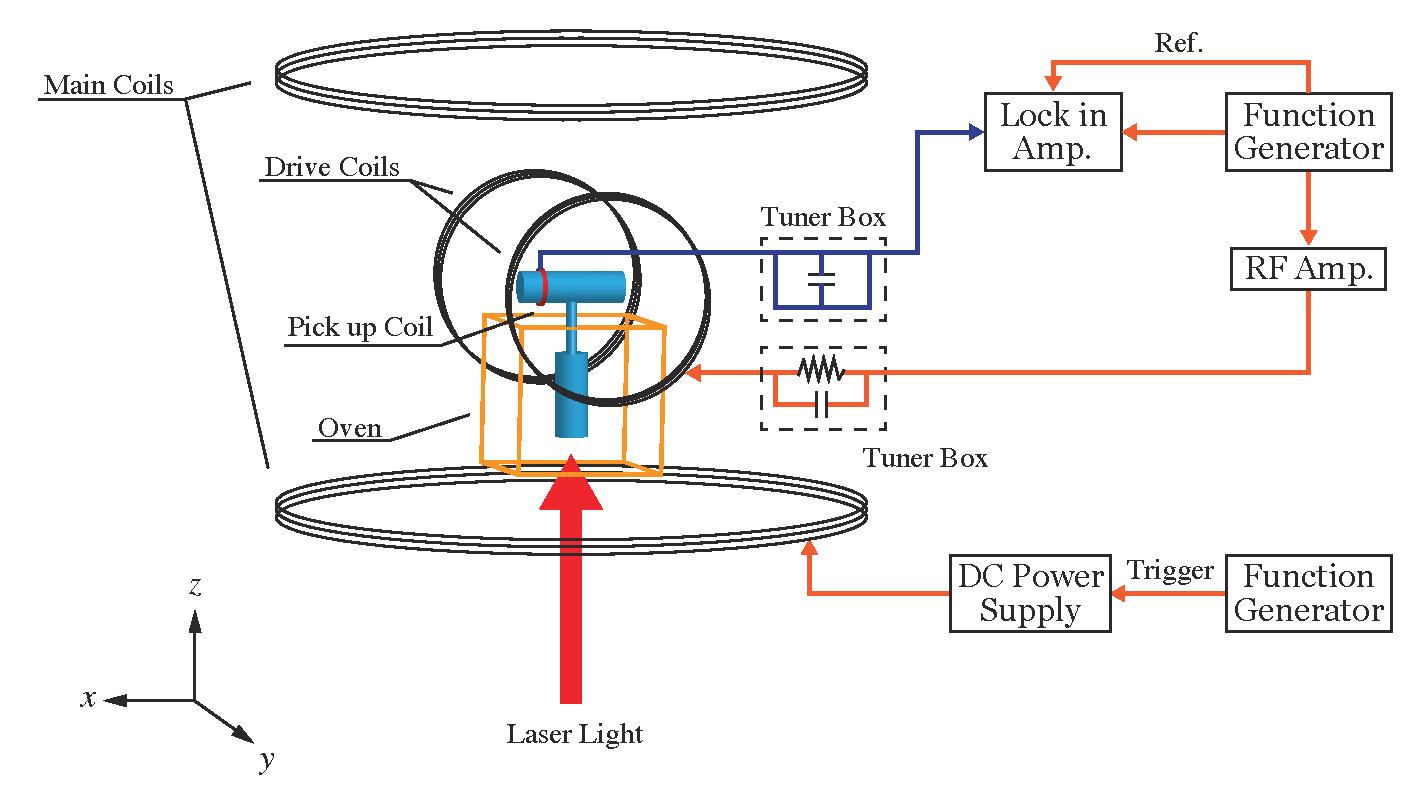
\includegraphics[clip, width=1.0\linewidth]{./chap3/fig/AFP-NMR_setup.pdf}\\
%  \caption{AFP-NMR装置の概略図}
%  \label{AFP-NMR}
% \end{figure}

% \begin{description}
%  \item[高周波磁場発生装置] \\
%  高周波磁場発生装置は、ファンクションジェネレーター(FG120, YOKOGAWA社)から出力された交流信号をRFアンプ(T145-4016A, THAMWAY社)によって増幅し、共振回路を通ってドライブコイルに印加することで高周波磁場を発生させる。\\
%  ドライブコイルは、標的セル周辺において均一な磁場を生成するために、メインコイルおよび補正コイルと同様にヘルムホルツ型のコイルとした。本研究におけるドライブコイルの仕様を表\ref{drive-coil_design}に示す。
% %
% \begin{table}[htbp]
%  \caption{本研究で使用したドライブコイルの仕様}
%  \centering
%   \begin{tabular}{|c|c|} \hline 
% 直径 & $45~{\rm cm}$ \\
% 導線の太さ & $\phi 1~{\rm mm}$ \\
% 巻き数 & $50$回 \\
% 抵抗 & $3.4~{\rm \Omega}$ \\
% インダクタンス & $6.1~{\rm mH}$ \\ \hline
%   \end{tabular}
%  \label{drive-coil_design}
% \end{table}
% %
% またドライブコイルの軸方向における磁場の大きさとドライブコイルに印加した直流電流との関係を図\ref{drive-coil}に示す。図\ref{drive-coil}のグラフは一次関数でフィッティングした結果を示しており、切片は測定した環境中の残留磁場によるものである。フィッティングの結果、ドライブコイルに流れる電流$I_{\rm drive}$と中心部におけるドライブコイルが作る磁場の大きさ$B_0$は
% %
% \begin{equation}
%  B_0~[{\rm mT}] = (0.203 \pm 0.010) \times I_{\rm drive}~[{\rm A}] + (0.056 \pm 0.006)
%  \label{B0-Idrive}
% \end{equation}
% %
% と表される。

% \begin{figure}[htbp]
%  \centering
%  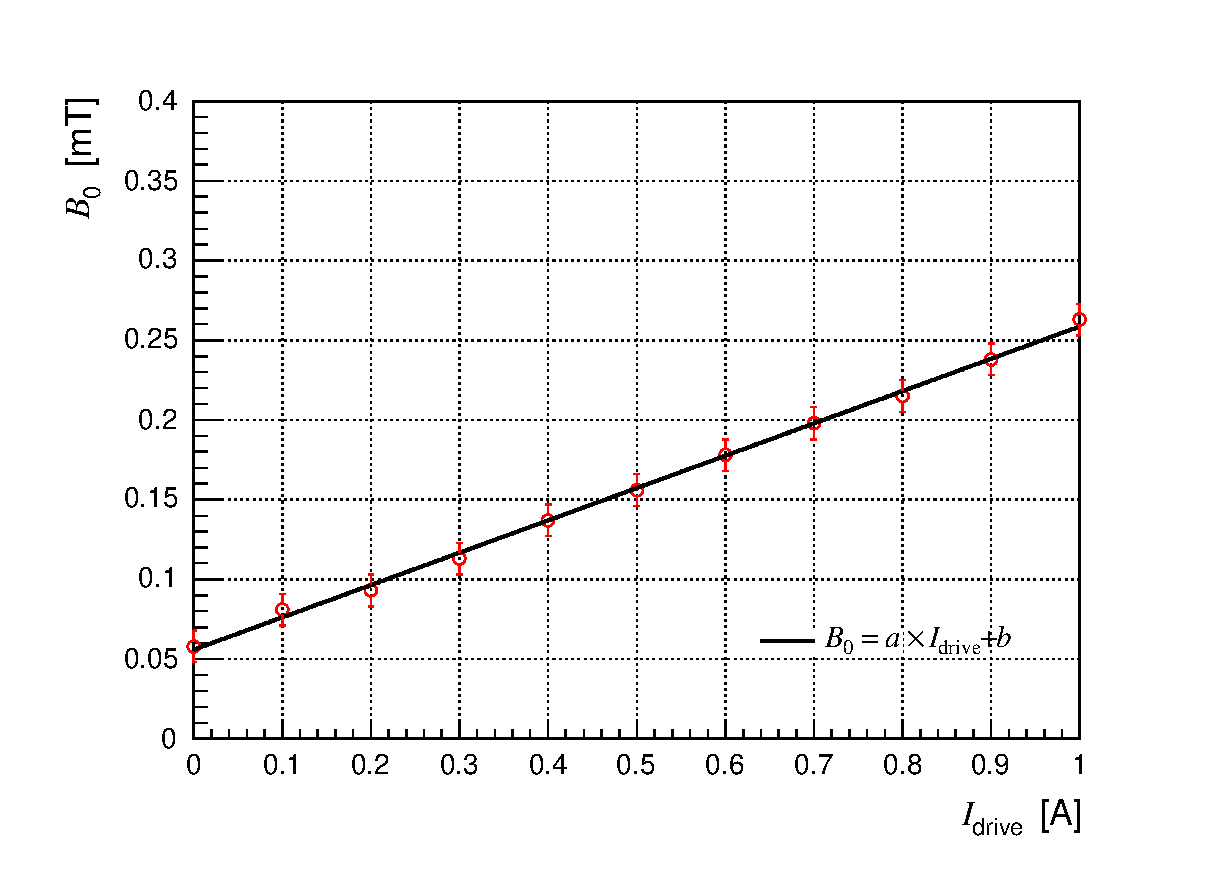
\includegraphics[clip, width=10cm]{./chap3/fig/Drive_Coil.eps}\\
%  \caption{ドライブコイルの励磁曲線}
%  \label{drive-coil}
% \end{figure}

%  メインコイルによって生成される静磁場の大きさは$1~{\rm mT}$程度なので、AFP条件からドライブコイルによって生成する振動磁場の振幅は$0.005〜0.010~{\rm mT}$程度が求められる。図\ref{drive-coil}におけるフィッティングの結果より、残留磁場の影響を無視すると、$0.005~{\rm mT}$程度の振幅を得るのに必要な印加電流はおよそ$25~{\rm mA}$となる。この条件を満たすために、ファンクションジェネレーターの出力信号をRFアンプおよび共振回路によって増幅させた。共振回路はドライブコイルに対して直列にコンデンサを入れた、直列共振回路(ドライブコイル用Tuner Box)を製作した。また印加電流値を読み取るために$10~{\rm \Omega}$の抵抗も組み込んだ。直列共振回路における共振周波数$f_0$は、次の式で書ける。
% %
% \begin{equation}
%  f_0 = \frac{\omega_0}{2 \pi} = \frac{1}{2 \pi \sqrt{LC}}
%  \label{series_reso}
% \end{equation}
% %
% ここで、$\omega_0$は共振角周波数、$L$はコイルのインダクタンスであり、$C$はコンデンサの電気容量である。仮に静磁場の大きさを$2.50~{\rm mT}$とした場合、式(\ref{B0_reso})よりNMRの共鳴周波数は
% %
% \begin{equation}
%  f_0 = \frac{2.50 \cdot 2.04 \times 10^5}{2 \pi} \simeq 81.2~[{\rm kHz}]
% \end{equation}
% %
% となる。式(\ref{series_reso})より、この共鳴周波数を得るために必要なコンデンサの電気容量は、表\ref{drive-coil_design}よりドライブコイルのインダクタンスが$L=6.1~{\rm mH}$であるから
% %
% \begin{eqnarray}
%  C &=& \frac{1}{(2 \pi f_0)^2 L} \nonumber \\
%  &=& \frac{1}{(2 \pi \cdot 81.2 \times 10^3)^2 \cdot 6.1 \times 10^{-3}} \nonumber \\
%  &\simeq& 0.630~[{\rm nF}]
% \end{eqnarray}
% %
% と求められる。実際は、回路系に含まれる浮遊容量等の影響があるので、計算値とは異なる値になると考えられる。\\
%  本研究で使用したドライブコイル用のTuner Boxの共振周波数測定結果を図\ref{drive-coil_tune}に示す。共振周波数の測定は、ドライブコイルに印加する電流の周波数を$0.5~{\rm kHz}$ずつ変化させつつ、Tuner Boxに組み込んだ抵抗の両端の電圧を読み取ることで行った。ファンクションジェネレーターの出力は$100~{\rm mV}$であり、コンデンサの電気容量は$0.253~{\rm nF}$とした。測定結果から、およそ$87~{\rm kHz}$の周波数において$25~{\rm mA}$以上の印加電流値が得られた。

% \begin{figure}[htbp]
%  \centering
%  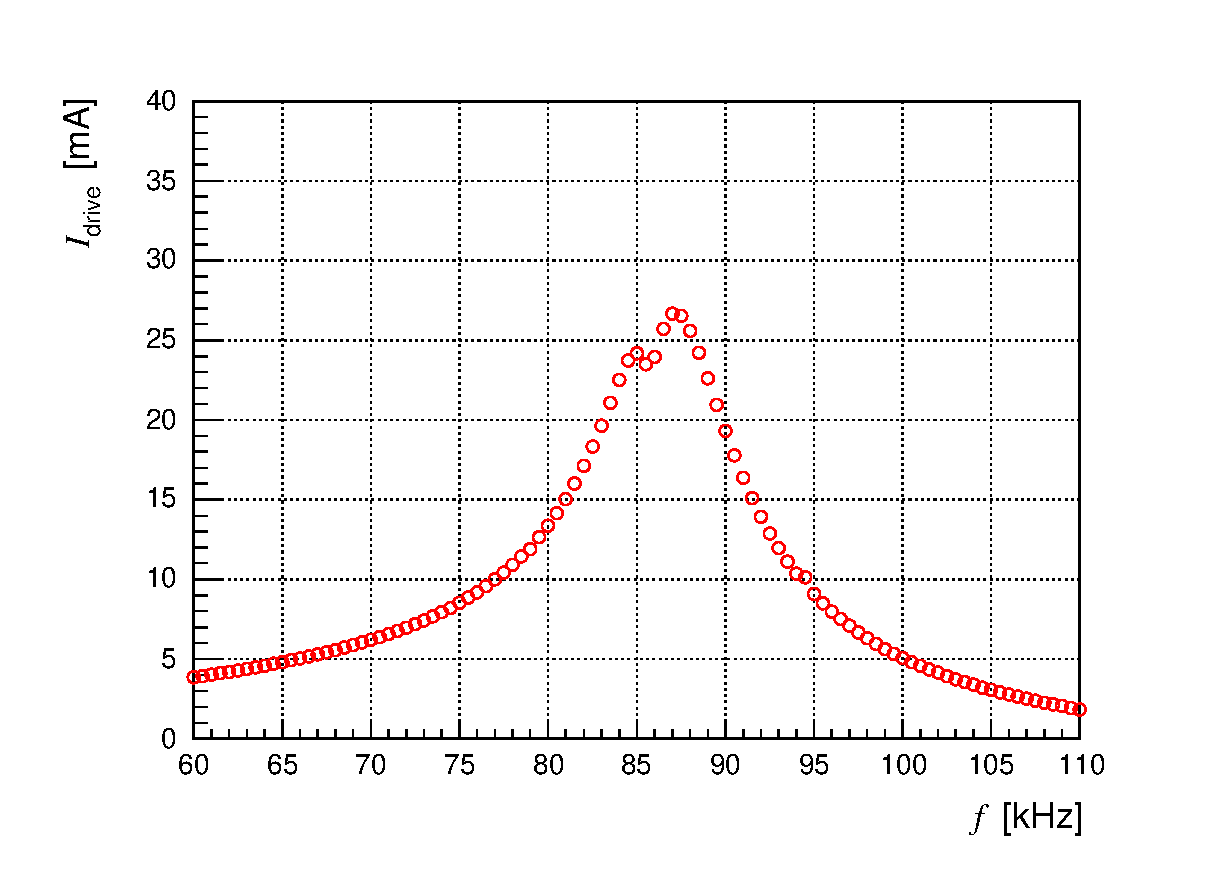
\includegraphics[clip, width=10cm]{./chap3/fig/Drive_Coil_tune.eps}\\
%  \caption{ドライブコイルの共振周波数測定。縦軸は実効値である。}
%  \label{drive-coil_tune}
% \end{figure}


%  \item[静磁場発生および掃引装置] \\
%  静磁場は、直流電源を用いてメインコイルに数 A程度の電流を流すことで発生させる。典型的な静磁場の大きさは$1〜3~{\rm mT}$である。今回使用した直流電源は、3.2.1節でも述べたようにTTL規格のトリガー信号を入力することで設定された二つの電流値の間を掃引できる。本研究では、ファンクションジェネレーターから$5~{\rm V}$のトリガー信号を直流電源に入力することで掃引を行った。また、ダイヤルによって磁場掃引時間を調整することができ、AFP条件を満たすような磁場の掃引速度を決定できる。本研究では磁場の掃引範囲として電流値を$2.50~{\rm A}$〜$5.95~{\rm A}$と設定した。これは磁場では$1.24~{\rm mT}$〜$2.96~{\rm mT}$に相当する。また掃引速度は、$1$秒あたり$0.19~{\rm A}$と設定した。

%  \item[NMR信号検出装置] \\
%  NMR信号検出装置は、偏極した$^3$He原子核集団が作る磁化を検出するためのピックアップコイル、信号を読み取るロックインアンプ(SR830, Stanford Research Systems社)、およびロックインアンプへ参照信号を入力するファンクションジェネレーターから構成される。\\
%  本研究で使用したピックアップコイルの仕様を表\ref{pick-coil_design}に示す。コイルの導線には$\phi 0.2~{\rm mm}$のエナメル線を使用し、$55$回巻きを四層重ねた$220$回巻きとした。また偏極した$^3$He原子核集団が作る磁化によってコイルに誘起される誘導電流を検出するために、回路系で得られる電圧が最大となるようにコンデンサを並列に組み込んだ並列共振回路(ピックアップコイル用Tuner Box)を製作した。コンデンサの電気容量は$0.08~{\rm nF}$とし、ドライブコイル用のTuner Boxと同様に共振周波数測定を行った。測定結果を図\ref{pick-coil_tune}に示す。この時、ピックアップコイルはドライブコイルと平行になるように設置し、ファンクションジェネレーターの出力は$100~{\rm mV}$とした。また測定時はドライブコイル用のTuner Boxを取り外し、抵抗のみを入れたものを組み込んだ。これにより、ドライブコイルに流れる電流が周波数に依らずほぼ一定となる。測定結果から、およそ$86~{\rm kHz}$において共振ピークが得られた。
% %
% \begin{table}[htbp]
%  \caption{ピックアップコイルの仕様}
%  \centering
%   \begin{tabular}{|c|c|} \hline 
% 直径 & $46~{\rm mm}$ \\
% 導線の太さ & $\phi 0.2~{\rm mm}$ \\
% 巻き数 & $220$回 \\
% 抵抗 & $21~{\rm \Omega}$ \\
% インダクタンス & $3.6~{\rm mH}$ \\ \hline
%   \end{tabular}
%  \label{pick-coil_design}
% \end{table}
% %

% \begin{figure}[tbp]
%  \centering
%  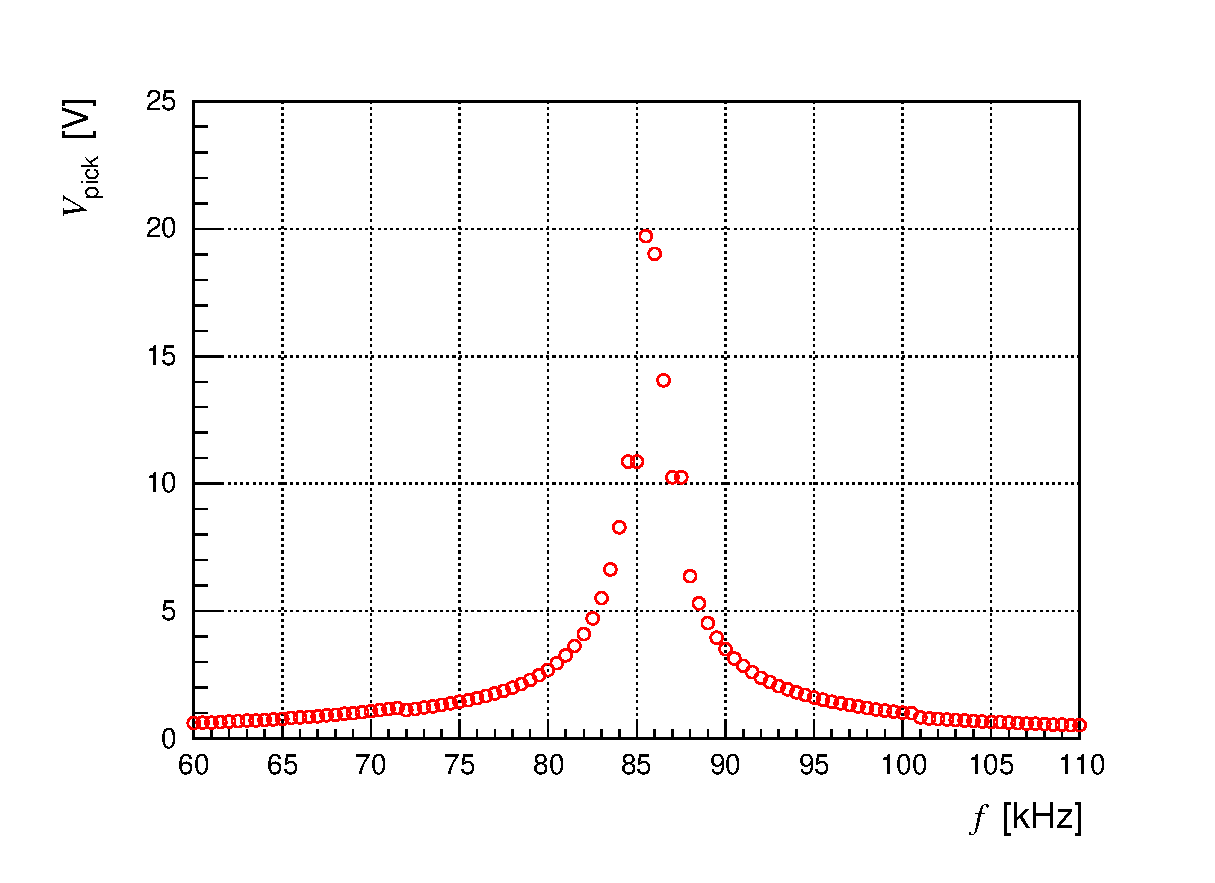
\includegraphics[clip, width=10cm]{./chap3/fig/Pickup_Coil_tune.eps}\\
%  \caption{ピックアップコイルの共振周波数測定。縦軸は実効値である。}
%  \label{pick-coil_tune}
% \end{figure}

%  ピックアップコイルに誘起されたNMR信号は、ロックインアンプを用いて測定した。ロックインアンプは特定の周波数成分の信号を取り出して増幅できる機器であり、ノイズに埋もれるような微小信号を非常に高感度で検出できる。これにより、式(\ref{V_pick})で表されるピックアップコイルに誘起される電圧の$\cos(\omega t)$の成分のみを取り出すことができる。以下に、ロックインアンプの測定原理について述べる。\\
%  ロックインアンプで取得したい信号$V_{\rm sig}(t)$を
% %
% \begin{equation}
%  V_{\rm sig}(t) = V_{\rm sig}^0 \cos(\omega_{\rm sig}t + \phi_{\rm sig})
%  \label{V_sig}
% \end{equation}
% %
% のように、周波数$\omega_{\rm sig}$をもつ周期関数とする。一般に、ロックインアンプへの入力信号には取得したい信号以外のバックグラウンドも含まれる。この取得したい信号に対し、ロックインアンプに参照信号として
% %
% \begin{equation}
%  V_{\rm ref}(t) = V_{\rm ref}^0 \cos(\omega_{\rm ref}t + \phi_{\rm ref})
%  \label{V_ref}
% \end{equation}
% %
% を入力する。ロックインアンプに入力された参照信号は、$90^\circ$位相シフト回路によって
% %
% \begin{eqnarray}
%  V_{\rm ref}^x(t) &=& V_{\rm ref}^0 \cos(\omega_{\rm ref}t + \phi_{\rm ref}) \\
%  V_{\rm ref}^y(t) &=& V_{\rm ref}^0 \sin(\omega_{\rm ref}t + \phi_{\rm ref})
% \end{eqnarray}
% %
% の二つの成分($x$成分および$y$成分)に分けられる。参照信号のこれらの成分を入力信号と積算させることにより
% %
% \begin{eqnarray}
%  V_x'(t) &=& V_{\rm sig}^0 \cos(\omega_{\rm sig}t + \phi_{\rm sig}) \times V_{\rm ref}^0 \cos(\omega_{\rm ref}t + \phi_{\rm ref}) \nonumber \\
%  &=& \frac{1}{2}V_{\rm sig}^0V_{\rm ref}^0 \{ \cos[(\omega_{\rm sig}-\omega_{\rm ref})t + (\phi_{\rm sig}-\phi_{\rm ref})] \nonumber \\
%  & & + \cos[(\omega_{\rm sig}+\omega_{\rm ref})t + (\phi_{\rm sig}+\phi_{\rm ref})] \}
% \end{eqnarray}
% %
% %
% \begin{eqnarray}
%  V_y'(t) &=& V_{\rm sig}^0 \cos(\omega_{\rm sig}t + \phi_{\rm sig}) \times V_{\rm ref}^0 \sin(\omega_{\rm ref}t + \phi_{\rm ref}) \nonumber \\
%  &=& \frac{1}{2}V_{\rm sig}^0V_{\rm ref}^0 \{ \sin[(\omega_{\rm sig}+\omega_{\rm ref})t + (\phi_{\rm sig}+\phi_{\rm ref})] \nonumber \\
%  & & - \sin[(\omega_{\rm sig}-\omega_{\rm ref})t + (\phi_{\rm sig}-\phi_{\rm ref})] \}
% \end{eqnarray}
% %
% となり、低周波(周波数:$\omega_{\rm sig}-\omega_{\rm ref}$)成分と高周波(周波数:$\omega_{\rm sig}+\omega_{\rm ref}$)成分をもつ直交した信号$V_x'(t)$および$V_y'(t)$が得られる。またロックインアンプにはローパスフィルターが内蔵されており、これによって高周波成分はキャンセルされる。よって、$\omega_{\rm sig} = \omega_{\rm ref}$となるような参照信号を用いることにより
% %
% \begin{eqnarray}
%  V_x &=& \frac{1}{2}V_{\rm sig}^0V_{\rm ref}^0 \cos(\phi_{\rm sig} - \phi_{\rm ref}) \\
%  V_y &=& -\frac{1}{2}V_{\rm sig}^0V_{\rm ref}^0 \sin(\phi_{\rm sig} - \phi_{\rm ref})
% \end{eqnarray}
% %
% のような直流電圧が得られる。また位相差$\phi_{\rm sig} - \phi_{\rm ref}$による影響を無くすために
% %
% \begin{equation}
%  V_R \equiv \sqrt{V_x^2 + V_y^2} = \frac{1}{2}V_{\rm sig}^0V_{\rm ref}^0
%  \label{V_R}
% \end{equation}
% %
% を演算することによって、位相差に依らない直流信号を得ることができる。以上の原理により、ピックアップコイルに誘起される偏極した$^3$He原子核集団が作る磁化起因のNMR信号を測定できる。

% \end{description}

% %%%%%%%

% %% 3.3.2 %%
%   \subsection{Rb-ESR測定装置}
% AFP-NMR法による測定のみでは、$^3$He偏極度の絶対値を求めることができない。そこで本研究では、AFP-NMR測定における$^3$He偏極度の絶対値較正を行うために、RbのESR周波数シフト測定による$^3$He偏極度測定システムを開発した。\\
%  RbのESR周波数シフト測定を行うためのRb-ESR測定装置の概略図を図\ref{Rb-ESR}に示す。標的オーブン内に設置されたESRコイルによって標的セルのポンピング部に振動磁場をかけてESRを誘起し、それによって光ポンピングにより励起されたRb原子を脱励起させる。その際に放出する$D_2$線($780~{\rm nm}$)をフォトダイオード(S2387-1010R, 浜松ホトニクス社)で観測することで、RbのESR測定を行う。この時、$D_2$線のみを観測するためにフォトダイオードの受光面の前面に$D_2$フィルター(VPFHT-12.5C-7800, シグマ光機社)を入れた。このフィルターの中心波長は$780~{\rm nm}$で、半値幅は$4.25~{\rm nm}$である。これにより、光ポンピングの円偏光レーザー(795~{\rm nm})の反射光等を遮断する。またフォトダイオードの信号はI-V変換器(T-IVA001BZ, TURTLE社)によって増幅させ、ロックインアンプに入力した。

% \begin{figure}[tbp]
%  \centering
%  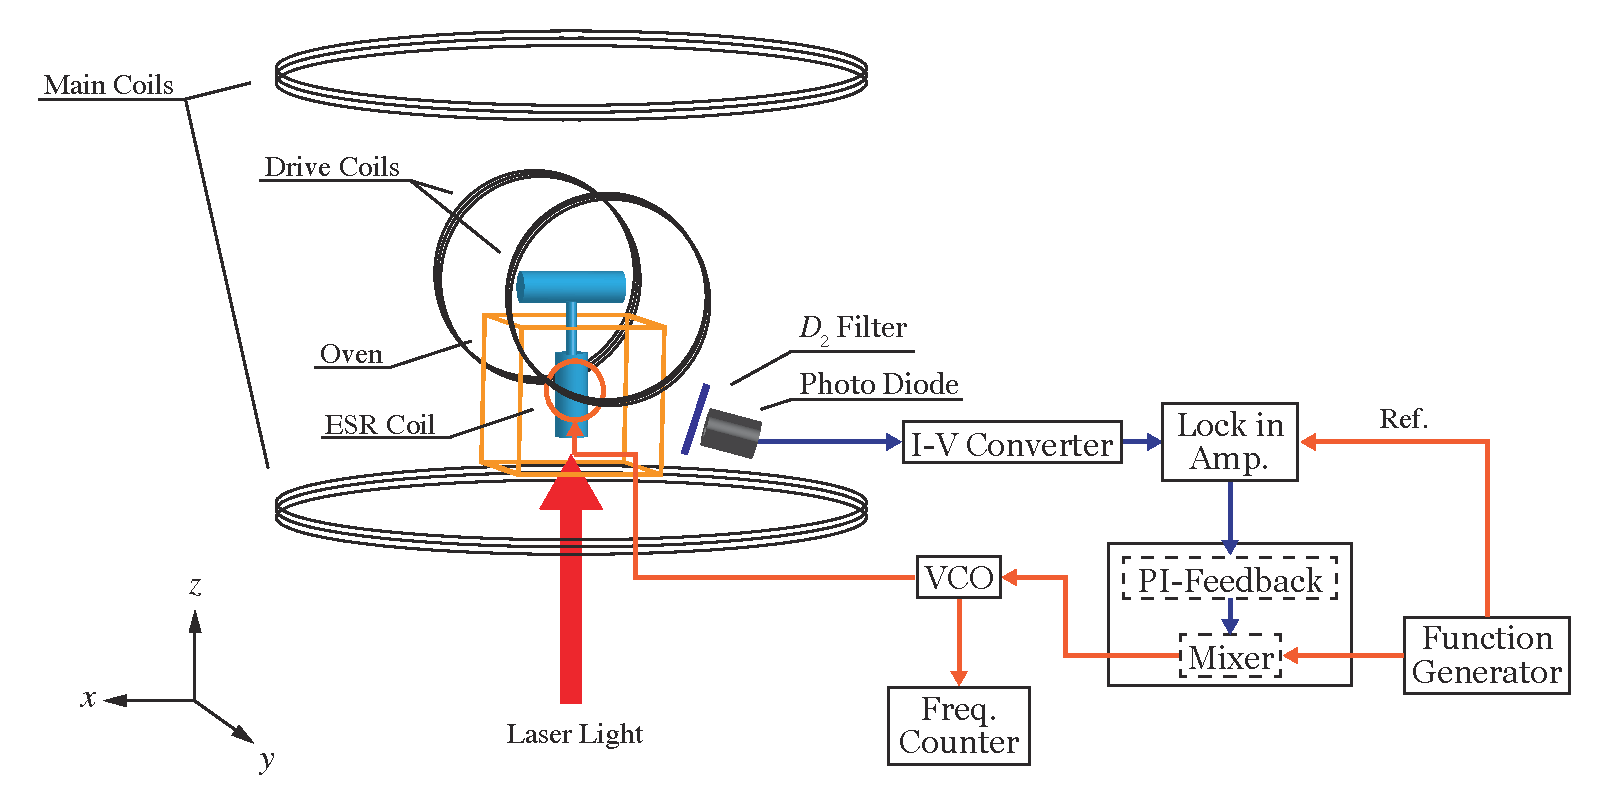
\includegraphics[clip, width=1.0\linewidth]{./chap3/fig/ESR_setup.pdf}\\
%  \caption{Rb-ESR測定装置の概略図}
%  \label{Rb-ESR}
% \end{figure}

% 振動磁場を印加するESRコイルは電圧制御発振器(VCO)に接続されている。VCOは入力信号の大きさに応じて発振する信号の周波数を制御できるもので、本研究ではVCOとしてHEWLETT PACKARD社製のHP8116Aを用いた。VCOへの制御入力信号としてsin波と直流電圧(offset)を用いることで、ESR周波数の前後で振動磁場の周波数を変調させることができる。本測定では、制御入力信号としてファンクションジェネレーター(33220A, Agilent社)の出力を用いた。出力するsin波の振幅は$60~{\rm mVpp}$、変調周波数は$120~{\rm Hz}$とした。またoffsetは$3~{\rm V}$程度とした。\\
%  ESR周波数は静磁場の大きさに依存するので、磁場のふらつきによってESR周波数もふらつくことが考えられる。そこで、振動磁場の周波数を常にESR周波数を中心として変調させるために、PI-フィードバック回路を組み込んだ。フォトダイオードの信号をロックインアンプに入力し、また参照信号として振動磁場と同様の周波数を持つ矩形波もファンクションジェネレーターからロックインアンプに入力する。この時のロックインアンプの$y$出力$V_y$を、ESR周波数からのずれを反映する信号としてPI-フィードバック回路へと入力し、適当な時定数で増幅させてミキサーへ入力する。ミキサーにはファンクションジェネレーターのsin波信号も入力されており、PI-フィードバック回路からの信号をこれに加えてVCOへと制御信号として入力する。振動磁場の周波数がESR周波数となっていれば$V_y=0$となるが、ESR周波数からずれていれば$V_y \neq 0$となる。振動磁場の周波数がESR周波数よりも低周波数側にずれた時は正のフィードバックを、高周波数側にずれた時は負のフィードバックをかけることで、振動磁場の周波数が常にESR周波数を中心として変調される。またこの時の振動磁場の周波数は、VCOの出力を周波数カウンター(TR5822, ADVANTEST社)に入力して測定した。周波数カウンターをLinuxコンピューターのGPIB制御によって動作させ、測定データをPCに取り込んだ。

% %%%%%%%
% %%%%%%%%%%
